\documentclass[aspectratio=169,hyperref={pdfpagelabels=false}]{beamer}
\input{dtutemplates/templates/Beamer/template/preamble}

\usepackage{array}
\usepackage{pgfpages}
\setbeameroption{show notes on second screen=right}
\usetikzlibrary{positioning}

\title{CAN/CAN~FD\\Protocol Controller}
\subtitle{Implementation and Verification in VHDL}
\author{Mads Richardt}
\date{June 11, 2026}

\setdepartment{DTU Compute}
\setcolor{dtured}

\def\figures{../docs/figures}

\begin{document}

\inserttitlepage

% ==========================================
% SLIDE 0: Industrial context
% ==========================================
\section{Introduction}
\begin{frame}{Industrial Collaboration}
	\begin{columns}[T]
		\begin{column}{0.45\textwidth}
			\fbox{
\includegraphics[width=\textwidth,keepaspectratio]{images/everllence_logo.png}}\\
			{\small\textit{Source: www.everllence.com}}
			\begin{itemize}
				\item  Everllence's principal activity is the design and maintenance of \textbf{marine propulsion systems}.
				\item Current CAN infrastructure at Everllence builds on the \textbf{CAN Classic protocol}
			\end{itemize}
		\end{column}
		\hfill
		\begin{column}{0.55\textwidth}
			\textbf{Project Context and Scope}
			\begin{itemize}\setlength{\itemsep}{6pt}
				\item The thesis was conducted within the Everllence's \textbf{engine control department}
				\item Everllence is \textbf{considering migrating current CAN infrastructure} from CAN Classic to CAN FD
				\item Pilot implementation of a \textbf{combined CAN Classic and CAN FD} protocol controller in VHDL, compatible with Everllence's existing CAN infrastructure
			\end{itemize}
		\end{column}
	\end{columns}
\end{frame}
\note{\footnotesize\begin{itemize}\setlength{\itemsep}{5pt}
		\item ``Everllence is a \textbf{Copenhagen-based} company. They build \textbf{marine propulsion systems} and run a custom \textbf{IO-extender FPGA} on the engine control bus that handles real-time motor telemetry and actuator commands.''
		\item ``The CAN controller currently runs as an \textbf{IP core on that FPGA}, operating at \textbf{500\,kbit/s} with a payload limit of \textbf{8 bytes per frame}.''
		\item ``This thesis was carried out within the engine control department, which \textbf{owns and maintains the CAN infrastructure} and initiated the migration evaluation.''
		\item ``The motivation is \textbf{future-proofing} --- as the platform evolves, \textbf{CAN FD} provides headroom with 64-byte payloads and up to 8\,Mbit/s, without changing the physical bus.''
		\item ``The thesis gives Everllence a \textbf{working reference implementation} --- a verified, ISO-compliant design they can use as a starting point and technical baseline for the full migration effort.''
	\end{itemize}}

% ==========================================
% SLIDE 1: What is CAN
% ==========================================
\begin{frame}{Controller Area Network (CAN) -- Key Attributes and Benefits}
	\begin{columns}[c]
		\begin{column}{0.60\textwidth}
			\fbox{
\includegraphics[width=\textwidth,keepaspectratio]{\figures/can_bus.png}}\\
			{\small\textit{Two-node CAN bus and node composition}}
		\end{column}
		\begin{column}{0.40\textwidth}
			\begin{itemize}\setlength{\itemsep}{10pt}
				\item \textbf{Simple and low cost:} Single shared multi-master bus, widely used in automotive and industrial contexts
				\item \textbf{Robust:} Differential signaling, built-in error detection, faulty nodes isolated
				\item \textbf{Priority-based access:} Highest priority ID wins bit-wise arbitration
			\end{itemize}
		\end{column}
	\end{columns}
\end{frame}
\note{\footnotesize\begin{itemize}
		\item So what is \textbf{CAN bus}? It is a \textbf{serial communication bus} developed by Bosch in the 1980s for connecting electronic control units in vehicles and industrial systems. The figure shows the physical setup of a two-node CAN bus --- each CAN node consists of a \textbf{CAN controller} handling the protocol logic and a \textbf{transceiver IC} driving the differential bus. All nodes share the same two wires, \textbf{CANH and CANL}, terminated at each end with a \textbf{120\,$\Omega$} resistor that matches the characteristic impedance of the twisted pair and prevents signal reflections.''
		\item \textbf{Simple and low cost:} ``Just \textbf{two wires} shared by all nodes, and every node can initiate a transfer --- no central master node required.
		\item \textbf{Robust:} The bus uses \textbf{differential signaling} on CANH and CANL, which makes it inherently noise-resistant. Faulty nodes are automatically isolated through the \textbf{bus-off} mechanism.
		\item \textbf{Priority-based access:} Arbitration is \textbf{non-destructive} -- the bus implements a \textbf{wired-AND} where dominant ('0') always beats recessive ('1'). A losing node backs off the moment it detects a stronger signal, leaving the winning frame \textbf{uninterrupted}.
	\end{itemize}}

% ==========================================
% SLIDE: Bit Timing
% ==========================================
\begin{frame}{CAN Bit Timing and Synchronization}
	\fbox{
\includegraphics[width=\textwidth,keepaspectratio]{\figures/bit_timing.png}}\\
	{\small\textit{CAN bit segmentation and sample point}}
	\begin{itemize}
		\item Receiving nodes do \textbf{hard synchronization} on the first frame bit and \textbf{resynchronization on recessive-to-dominant} edges mid-frame
	\end{itemize}
\end{frame}
\note{\footnotesize\begin{itemize}
		\item Each node on the bus runs on its own \textbf{independent clock oscillator} so the bus needs a way to synchronize nodes and correct for oscillator drift during transmission.
		\item The synchronization mechanism is comprised of two sycn types: Hard sync and resync. \textbf{Hard sync} align node clocks by resetting the timer logic at the start of each frame. \textbf{Resynchronization} corrects for oscillator drift mid-frame by lengthening Phase\_Seg1 or shortening Phase\_Seg2 on recessive-to-dominant edge.
		\item ``The figure shows the bit segmentation of two nodes with node B synchronised to node A -- the bit edge of node A arrives within the sync\_seg of node B. Each bit is split into \textbf{Sync\_Seg}, \textbf{Prop\_Seg}, \textbf{Phase\_Seg1}, and \textbf{Phase\_Seg2}, with the \textbf{sample point} at the end of Phase\_Seg1. The leading node A is offset from B by the \textbf{one-way propagation delay}. Prop\_Seg must cover the full round-trip delay so A sees the settled bus level before sampling.''
	\end{itemize}}

% ==========================================
% SLIDE: Error Detection and Confinement
% ==========================================
\begin{frame}{Error Detection and Confinement}
	\begin{columns}[T]
		\begin{column}{0.60\textwidth}
			\textbf{Five error types}:
			\begin{itemize}\setlength{\itemsep}{3pt}
				\item \textbf{Bit:} transmitted bit $\neq$ monitored bus level
				\item \textbf{Stuff:} six consecutive identical bits detected
				\item \textbf{CRC:} computed vs.\ received remainder mismatch
				\item \textbf{Form:} fixed-form field violated
				\item \textbf{ACK:} no dominant ACK received
			\end{itemize}
			Any \textbf{detecting node sends an error flag} -- 6 dominant bits (error active) or 6 recessive bits (error passive)
		\end{column}
		\begin{column}{0.40\textwidth}
			\fbox{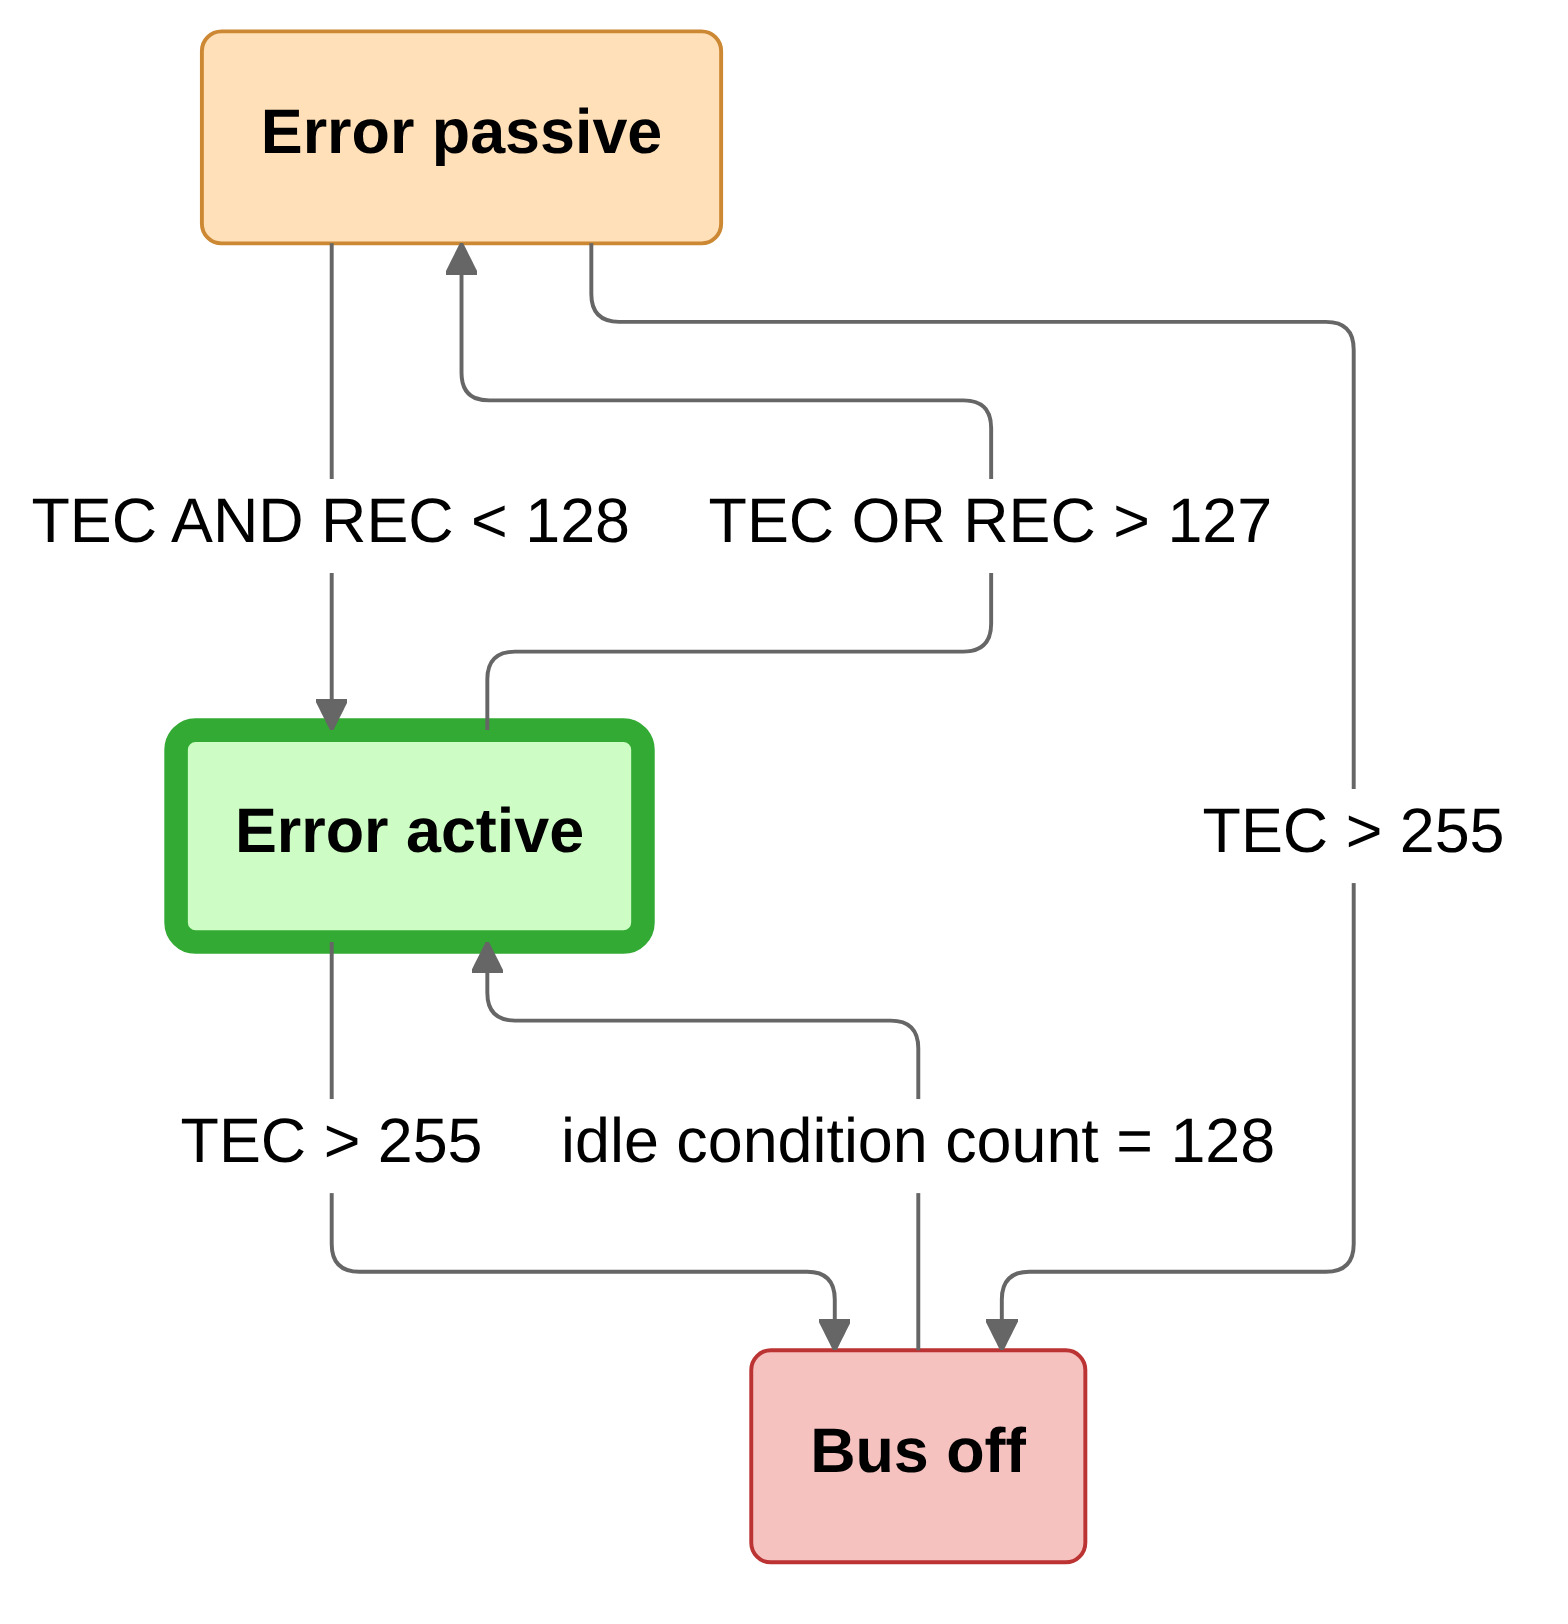
\includegraphics[width=\textwidth,keepaspectratio]{images/fce_simple.png}}\\
			{\small\textit{Fault confinement FSM}}
		\end{column}
	\end{columns}
\end{frame}
\note{\footnotesize\begin{itemize}\setlength{\itemsep}{5pt}
		\item ``This slide covers two related things --- the \textbf{five ways a CAN frame can go wrong}, and how the node reacts when errors accumulate.''
		\item \textbf{Five error types / error flag:} ``Any detecting node immediately sends an \textbf{error flag}. An \textbf{error active} node sends 6 dominant bits --- this violates the stuff rule and forces all other nodes to join in. An \textbf{error passive} node sends 6 recessive bits, which are invisible to other nodes --- the frame is not destroyed.''
		\item \textbf{Fault confinement FSM:} ``Each node independently tracks a \textbf{transmit error counter} (TEC) and \textbf{receive error counter} (REC). TEC goes up by 8 on a TX error and down by 1 on success. The FSM has three states --- \textbf{error active}, \textbf{error passive}, and \textbf{bus off} --- driven by these counters.''
		\item \textbf{Bus off:} ``Once TEC exceeds 255 the node stops driving entirely. Recovery requires seeing \textbf{128 sequences of 11 consecutive recessive bits} --- a deliberately long quiet period before re-joining the bus.''
	\end{itemize}}

% ==========================================
% SLIDE: CAN vs CAN FD
% ==========================================
\begin{frame}{CAN Classic (CC) vs. CAN Flexible Data Rate (CF)}
	\fbox{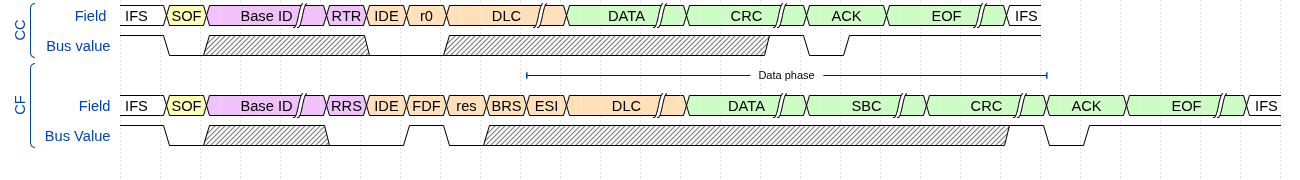
\includegraphics[width=\textwidth,keepaspectratio]{images/frame_format.png}}\\
	{\small\textit{CAN Classic and CAN FD frame structures}}
	\linebreak

	\footnotesize
	\begin{tabular}{p{0.30\textwidth} p{0.30\textwidth} p{0.30\textwidth}}
		\toprule
		Feature                      & CAN Classic                      & CAN FD                       \\
		\midrule
		Max bit rate                 & 1\,Mbit/s                        & 8\,Mbit/s (data phase)       \\
		Max payload                  & 8\,bytes                         & 64\,bytes                    \\
		Error detection HD$^\dagger$ & 6 typical, \textbf{2 worst case} & 6, all patterns, $\leq$64\,B \\
		Burst error detection        & up to 15\,bits                   & up to 17/21\,bits            \\
		\bottomrule
	\end{tabular}\\
	{\tiny $^\dagger$ CAN in Automation (CiA), \textit{CRC in CAN Frames}, can-cia.org.}
\end{frame}
\note{\footnotesize\begin{itemize}
		\item This slide compares \textbf{CAN Classic and CAN FD} --- the two frame formats this controller supports.
		\item The figure shows the two frame structures side by side. CAN FD adds the \textbf{BRS bit} (bit rate switch), \textbf{ESI} (error state indicator), and a \textbf{longer CRC field} to support the higher data rate and larger payload.
		\item \textbf{Max bit rate / payload:} CAN Classic tops out at \textbf{1\,Mbit/s} and \textbf{8 bytes}. CAN FD switches to up to \textbf{8\,Mbit/s} in the data phase and supports up to \textbf{64 bytes}.
		\item \textbf{Error detection HD:} CAN Classic computes CRC before stuffing, so two errors can \textbf{relocate a stuff bit} making the true and corrupted frames produce the \textbf{same CRC remainder}, giving \textbf{HD=2}. CAN FD includes stuff bits in the CRC and adds the \textbf{SBC field}, so any relocation changes the remainder and \textbf{restoring HD=6}.
		\item \textbf{Burst error detection:} Any burst of length $b < \deg(G)$ produces a polynomial the generator cannot divide --- so \textbf{CRC-15 catches all 15-bit bursts} for free. CAN FD uses \textbf{CRC-17/21} to both raise the burst ceiling and maintain \textbf{HD=6} over the larger 64-byte payloads.
	\end{itemize}}

% ==========================================
% SLIDE 2: Why clean-slate
% ==========================================
\begin{frame}{Project Objectives and Rationale}
	\begin{columns}[T]
		\begin{column}{0.50\textwidth}
			\textbf{Objectives}
			\begin{enumerate}
				\item Implement a CAN Classic/FD protocol controller in VHDL, compliant with ISO\,11898-1
				\item Structured requirements framework with traceability from ISO\,11898-1 to testbench evidence
				\item RTL design integrated via Avalon-ST into Everllence's existing FPGA infrastructure
			\end{enumerate}
		\end{column}
		\begin{column}{0.50\textwidth}
			\textbf{Why design in-house}
			\begin{itemize}
				\item \textbf{IP ownership:} 30-year service horizon
				\item \textbf{Verification authority:} own the test suite
				\item \textbf{Integration:} Avalon-ST + existing infrastructure
				\item \textbf{Platform independence:} portable VHDL-93
			\end{itemize}
		\end{column}
	\end{columns}
\end{frame}
\note{\footnotesize\begin{itemize}
		\item That covers the \textbf{CAN protocol background}. Now let's look at the \textbf{project objectives} and why Everllence chose to build the controller in-house rather than use a third-party IP core.
		\item \textbf{Objectives:} Three concrete goals -- a \textbf{verified ISO-compliant controller} in VHDL, a \textbf{structured requirements framework} with traceability from spec to test evidence, and \textbf{Avalon-ST integration} into the existing FPGA infrastructure.
		\item \textbf{IP ownership:} A \textbf{30-year service horizon} makes vendor dependency a real risk. Owning the RTL means the design can be maintained, ported, and extended without licensing constraints.
		\item \textbf{Verification authority:} Inheriting a third-party core means inheriting its test suite. Everllence needs to \textbf{own the verification} to know exactly what has and hasn't been tested.
		\item \textbf{Integration:} A clean-slate design with \textbf{Avalon-ST interfaces} fits directly into Everllence's existing FPGA infrastructure without adaptation layers.
		\item \textbf{Platform independence:} The design is in \textbf{portable VHDL-93} making it independent of any vendor-specific toolchains, which matters for a 30-year horizon.
	\end{itemize}}

% ==========================================
% SLIDE: Requirements extraction
% ==========================================
\section{Design and Implementation}
\begin{frame}{From ISO specification to Structured Requirements Set}
	\begin{columns}[c]
		\begin{column}{0.40\textwidth}
			\begin{itemize}\setlength{\itemsep}{8pt}
				\item \textbf{37 requirements} distilled from ISO\,11898-1:2024
				\item \textbf{\texttt{layer} field maps each requirement to an ISO reference model sub-layer}. This settled the module scope before any RTL was written
			\end{itemize}
		\end{column}
		\begin{column}{0.60\textwidth}
			\footnotesize
			\begin{tabular}{p{0.30\textwidth} p{0.6\textwidth}}
				\toprule
				\textbf{Field} & \textbf{Content}               \\
				\midrule
				id             & REQ-NNN                        \\
				source\_clause & ISO\,11898-1 section reference \\
				paraphrase     & Concise restatement            \\
				layer          & LLC / MAC / PCS / FCE / System \\
				priority       & P1 / P2 / P3                   \\
				\bottomrule
			\end{tabular}\\
			{\small\textit{Requirements table field descriptions}}
		\end{column}
	\end{columns}
\end{frame}
\note{\footnotesize\begin{itemize}
		\item Now let's focus on the \textbf{design and implementation} --- starting with how the ISO spec was turned into a structured requirements set.
		\item \textbf{37 requirements:} ISO\,11898-1 is a relatively sprawling document with requirements scattered across subsections and compound clauses and intermixed with descriptive language. So to make the requirement extraction more systematic and consistent the standard was converted to Markdown and fed to a Claude agent, which was prompted to extract all normative statements -- yielding \textbf{168 raw statements}. Manual review then distilled these to \textbf{37 verifiable requirements}.
		\item The table shows the dimensions along which the requirements were classified. \textbf{id} for traceability, \textbf{source\_clause} links back to the ISO section, \textbf{layer} assigns each requirement to a model sub-layer, and \textbf{priority} where P1,P2,P3 map to must-have, nice-to-have and optional according to the ISO standard.
		\item \textbf{\texttt{layer} field:} Each requirement is tagged with the ISO reference model sub-layer that owns it -- LLC, MAC, PCS, FCE, or System. The design was split along these boundaries thus settling the module scope before any RTL was written. System-tagged requirements pertain to the complete system and can not be verified at the sub-module level.
	\end{itemize}}

% ==========================================
% SLIDE: Layered architecture
% ==========================================
\begin{frame}{From ISO Reference Model to RTL Modules}
	\begin{columns}[c]
		\begin{column}{0.50\textwidth}
			\begin{center}
				\fbox{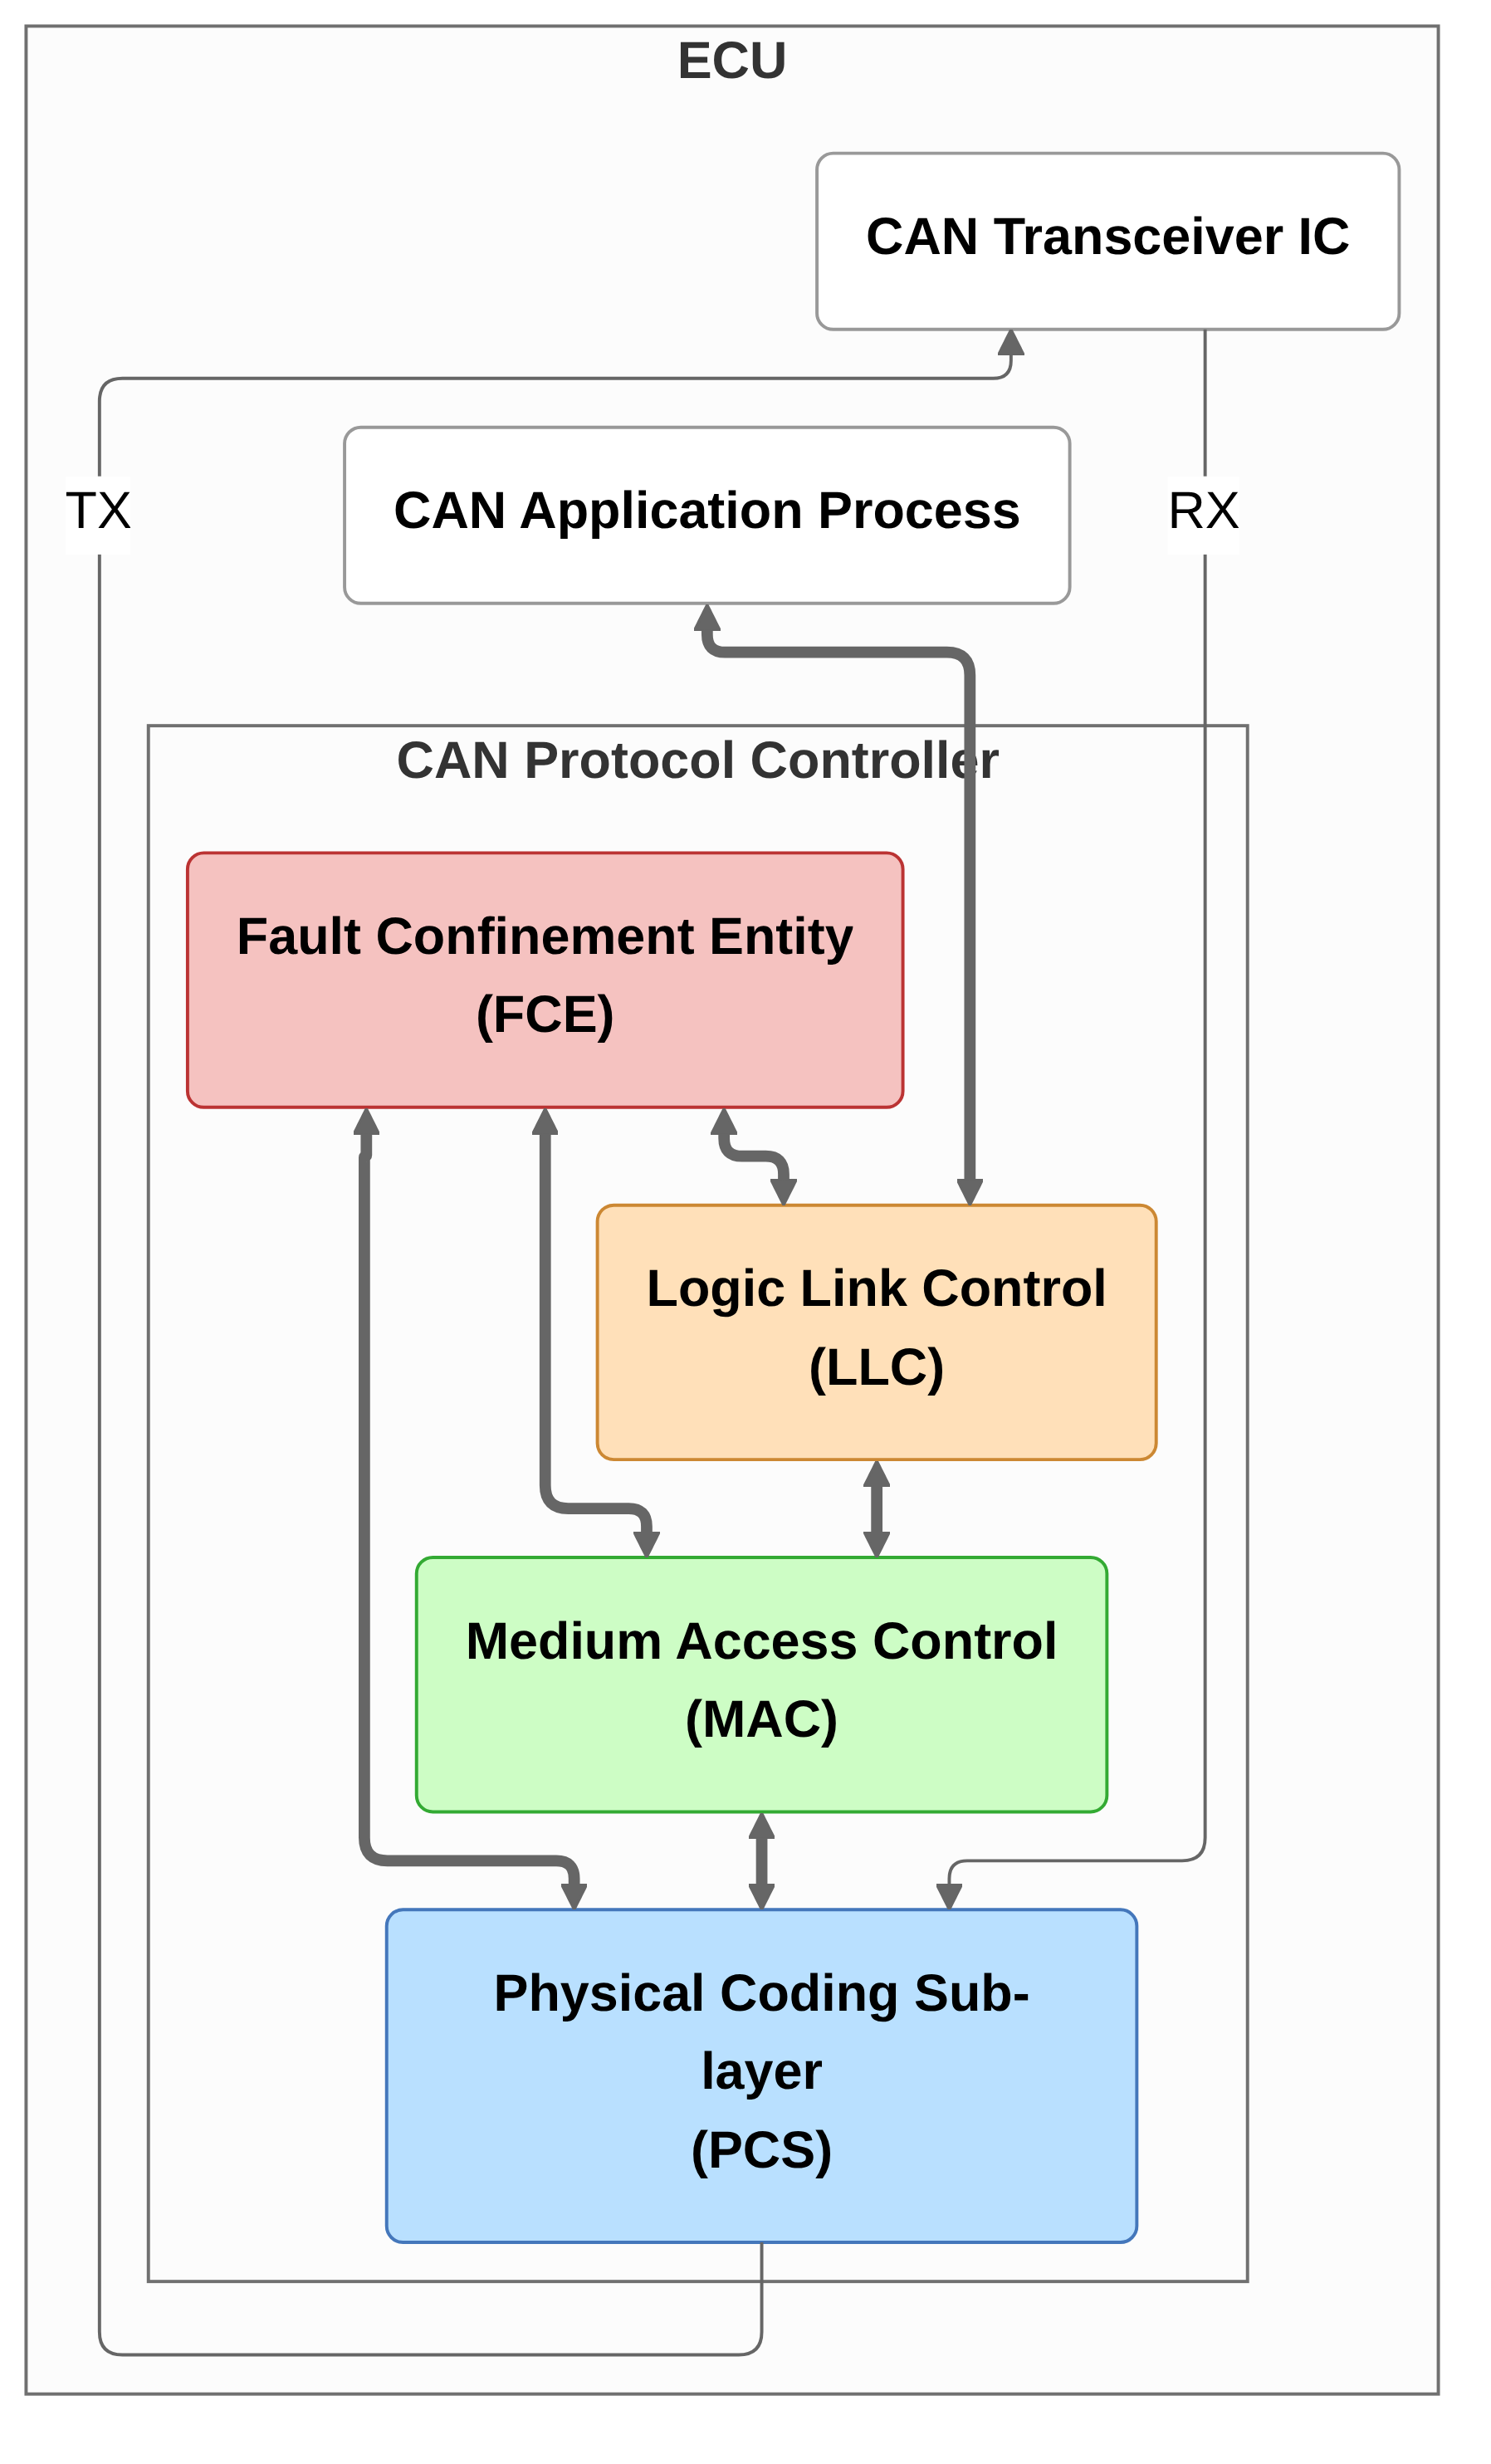
\includegraphics[height=0.75\textheight,keepaspectratio]{images/ecu.png}}\\{\small ISO\,11898-1 reference model}
			\end{center}
		\end{column}
		\begin{column}{0.50\textwidth}
			\begin{center}
				\fbox{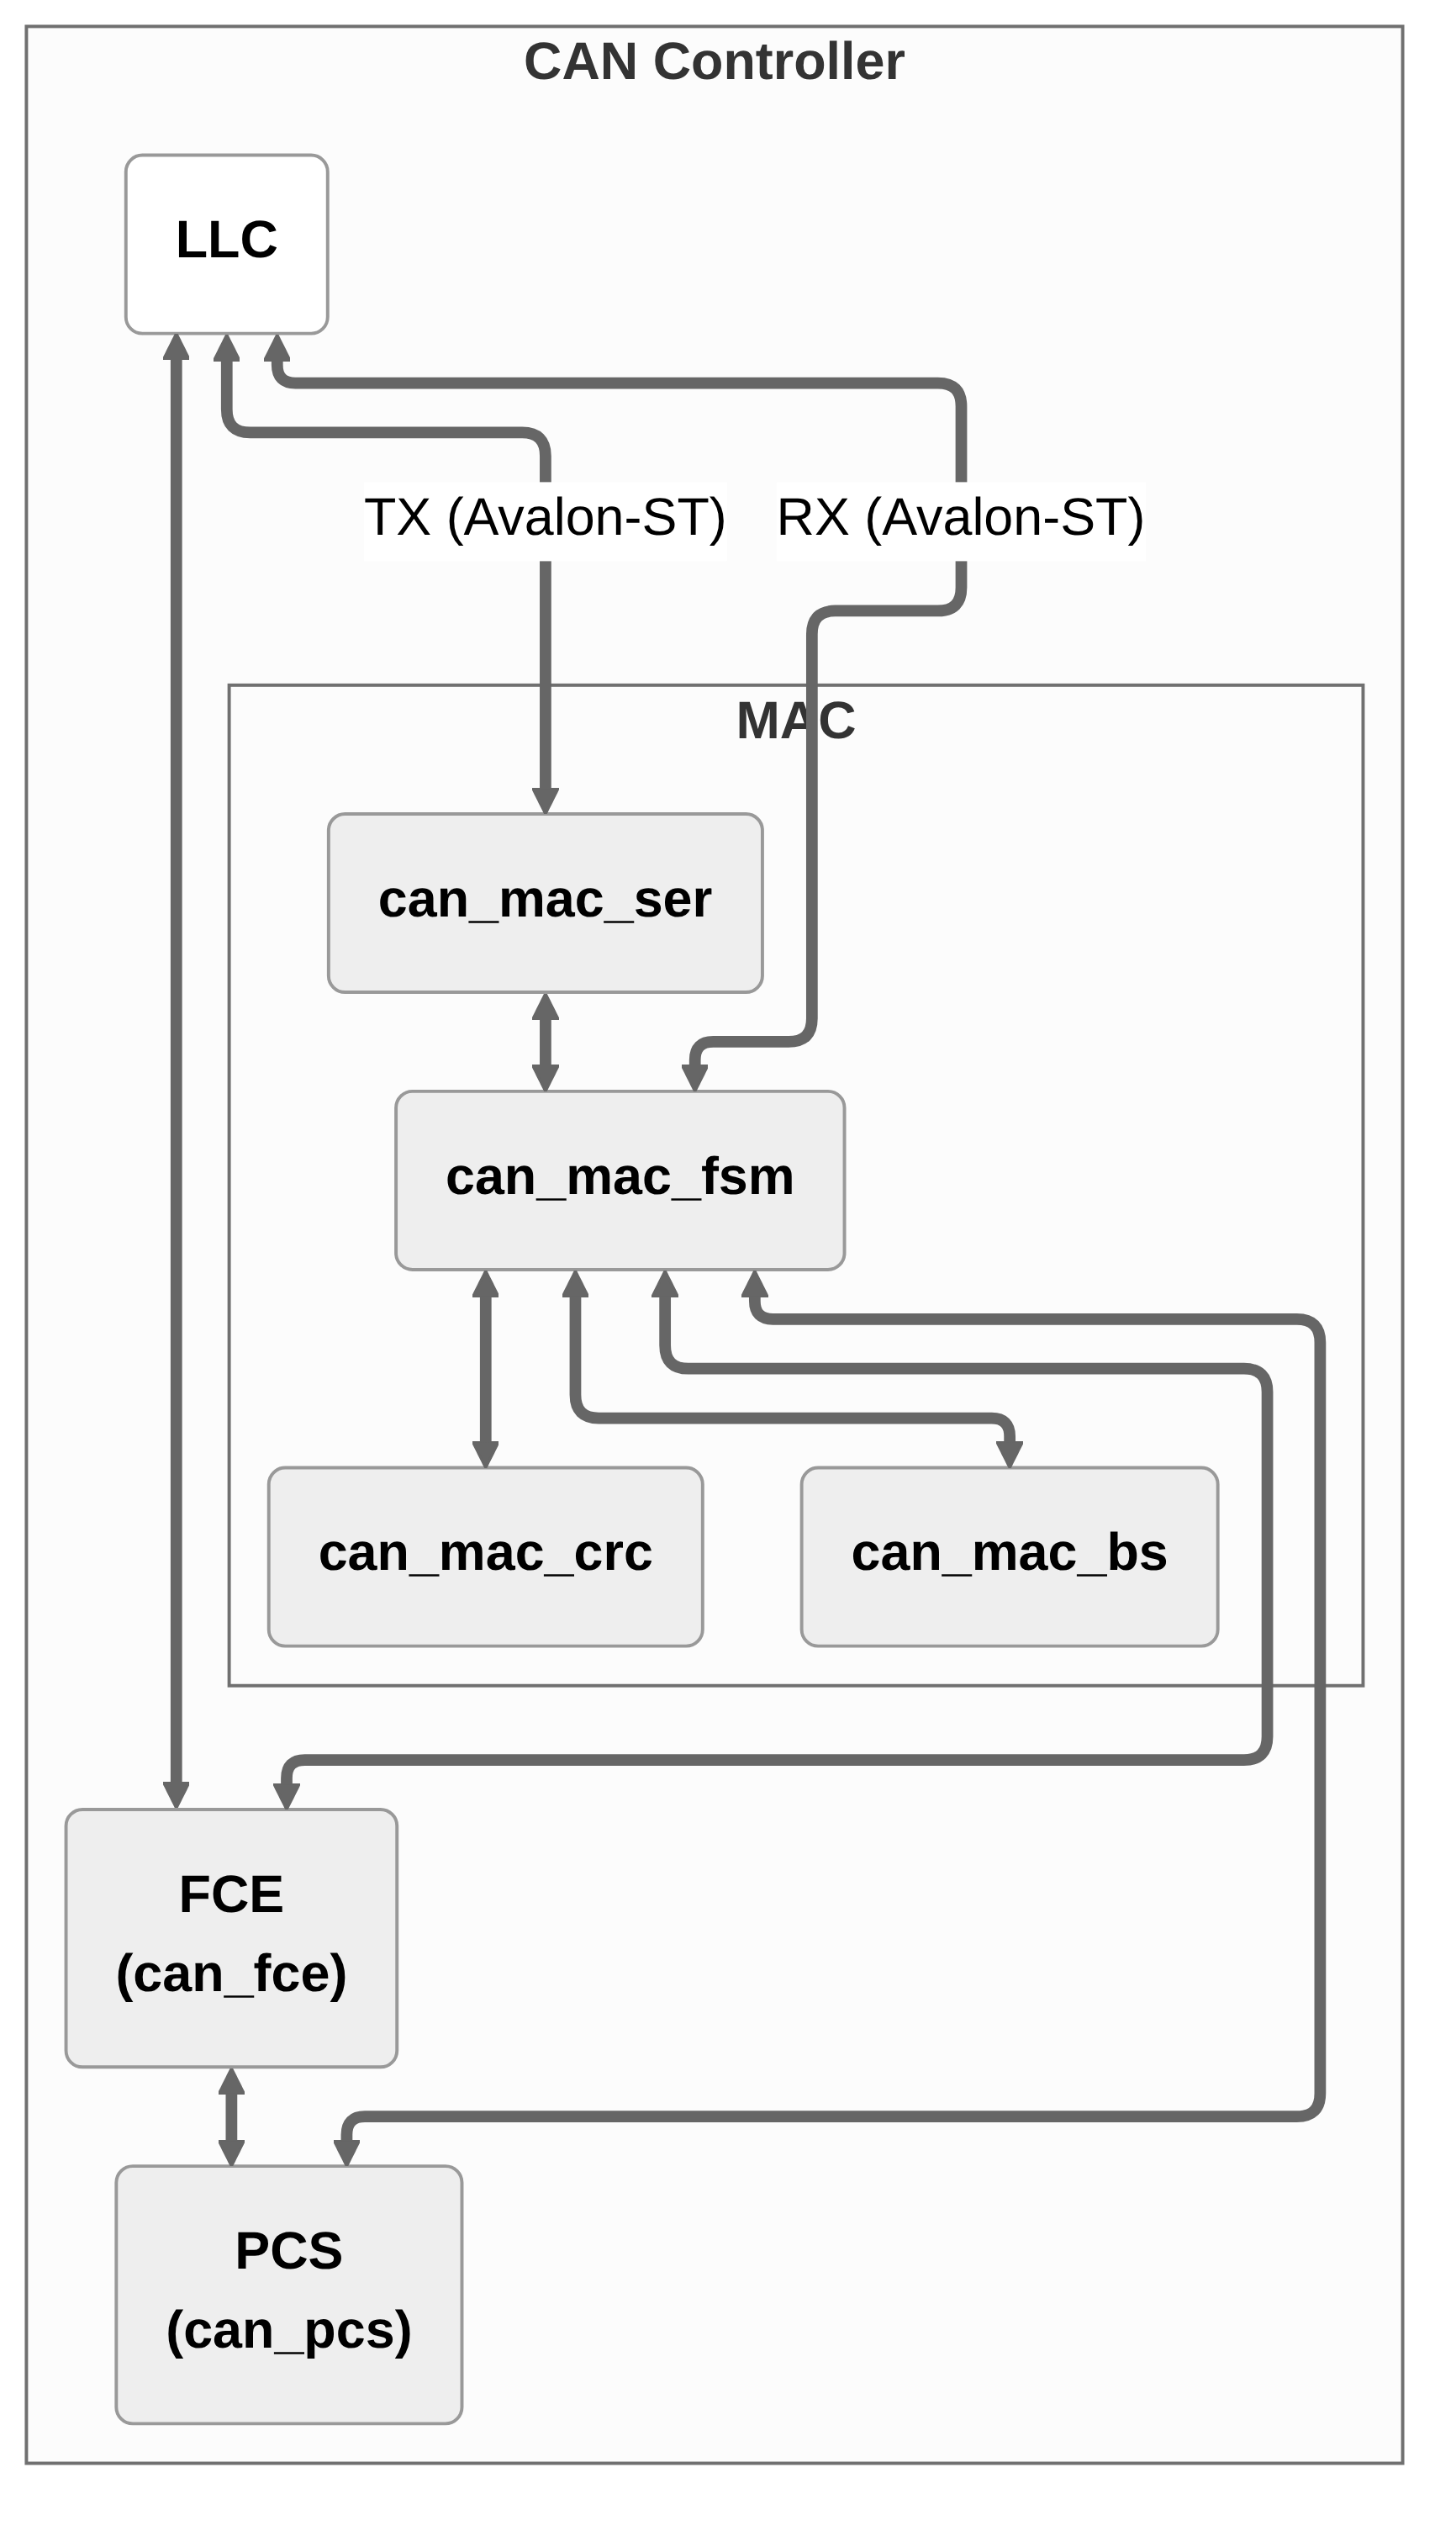
\includegraphics[height=0.75\textheight,keepaspectratio]{images/can_controller.png}}\\{\small Implemented RTL modules}
			\end{center}
		\end{column}
	\end{columns}
\end{frame}
\note{\footnotesize\begin{itemize}
		\item So this is the \textbf{ISO 11898-1 reference model} on the left and the \textbf{implemented RTL module structure} on the right. Each sub-layer maps directly to one or more RTL modules.
		\item \textbf{LLC} (Logic Link Control): The application-facing layer responsible for \textbf{acceptance filtering and frame retransmission}. This module was \textbf{deferred due to time constraints}. Without LLC the controller still transmits and receives fully compliant frames, but the host must handles filtering and retransmission directly. This works in practice because \textbf{both the LLC-MAC and LLC-host interfaces are Avalon-ST}, so the host can talk directly to the MAC using the same interface convention Everllence's existing infrastructure already speaks.
		\item \textbf{MAC} (Medium Access Control): orchestrates frame TX and RX, bit stuffing/destuffing, CRC, and bus arbitration. \textbf{Split into four sub-modules}: \texttt{can\_mac\_fsm} orchestrates, \texttt{can\_mac\_ser} serializes TX, \texttt{can\_mac\_bs} handles stuffing, \texttt{can\_mac\_crc} runs the CRC engines.
		\item \textbf{PCS} (Physical Coding Sub-layer): Responsible bit timing and clock synchronization.
		\item \textbf{FCE} (Fault Confinement Entity): Tracks transmitter/receiver errors and manages error state transitions.
	\end{itemize}}

% ==========================================
% SLIDE MAC-1: FSM per-field structure
% ==========================================
\begin{frame}{MAC: \texttt{can\_mac\_fsm} -- FSM orchestrating the MAC layer}
	\begin{columns}[c]
		\begin{column}{0.60\textwidth}
			\begin{itemize}\setlength{\itemsep}{8pt}
				\item The FSM State graph maps directly to the frame field sequence with one state per field and branching where CAN Classic and CAN FD formats diverge.
				\item An \texttt{is\_transmitter} flag gates TX vs.\ RX logic within each state.
				\item State transition on the sample point strobe from \texttt{can\_pcs}.
				\item Valid received frames are streamed to the LLC by a separate Avalon-ST interface control process, \texttt{p\_stream}.
			\end{itemize}
		\end{column}
		\begin{column}{0.40\textwidth}
			\begin{center}
				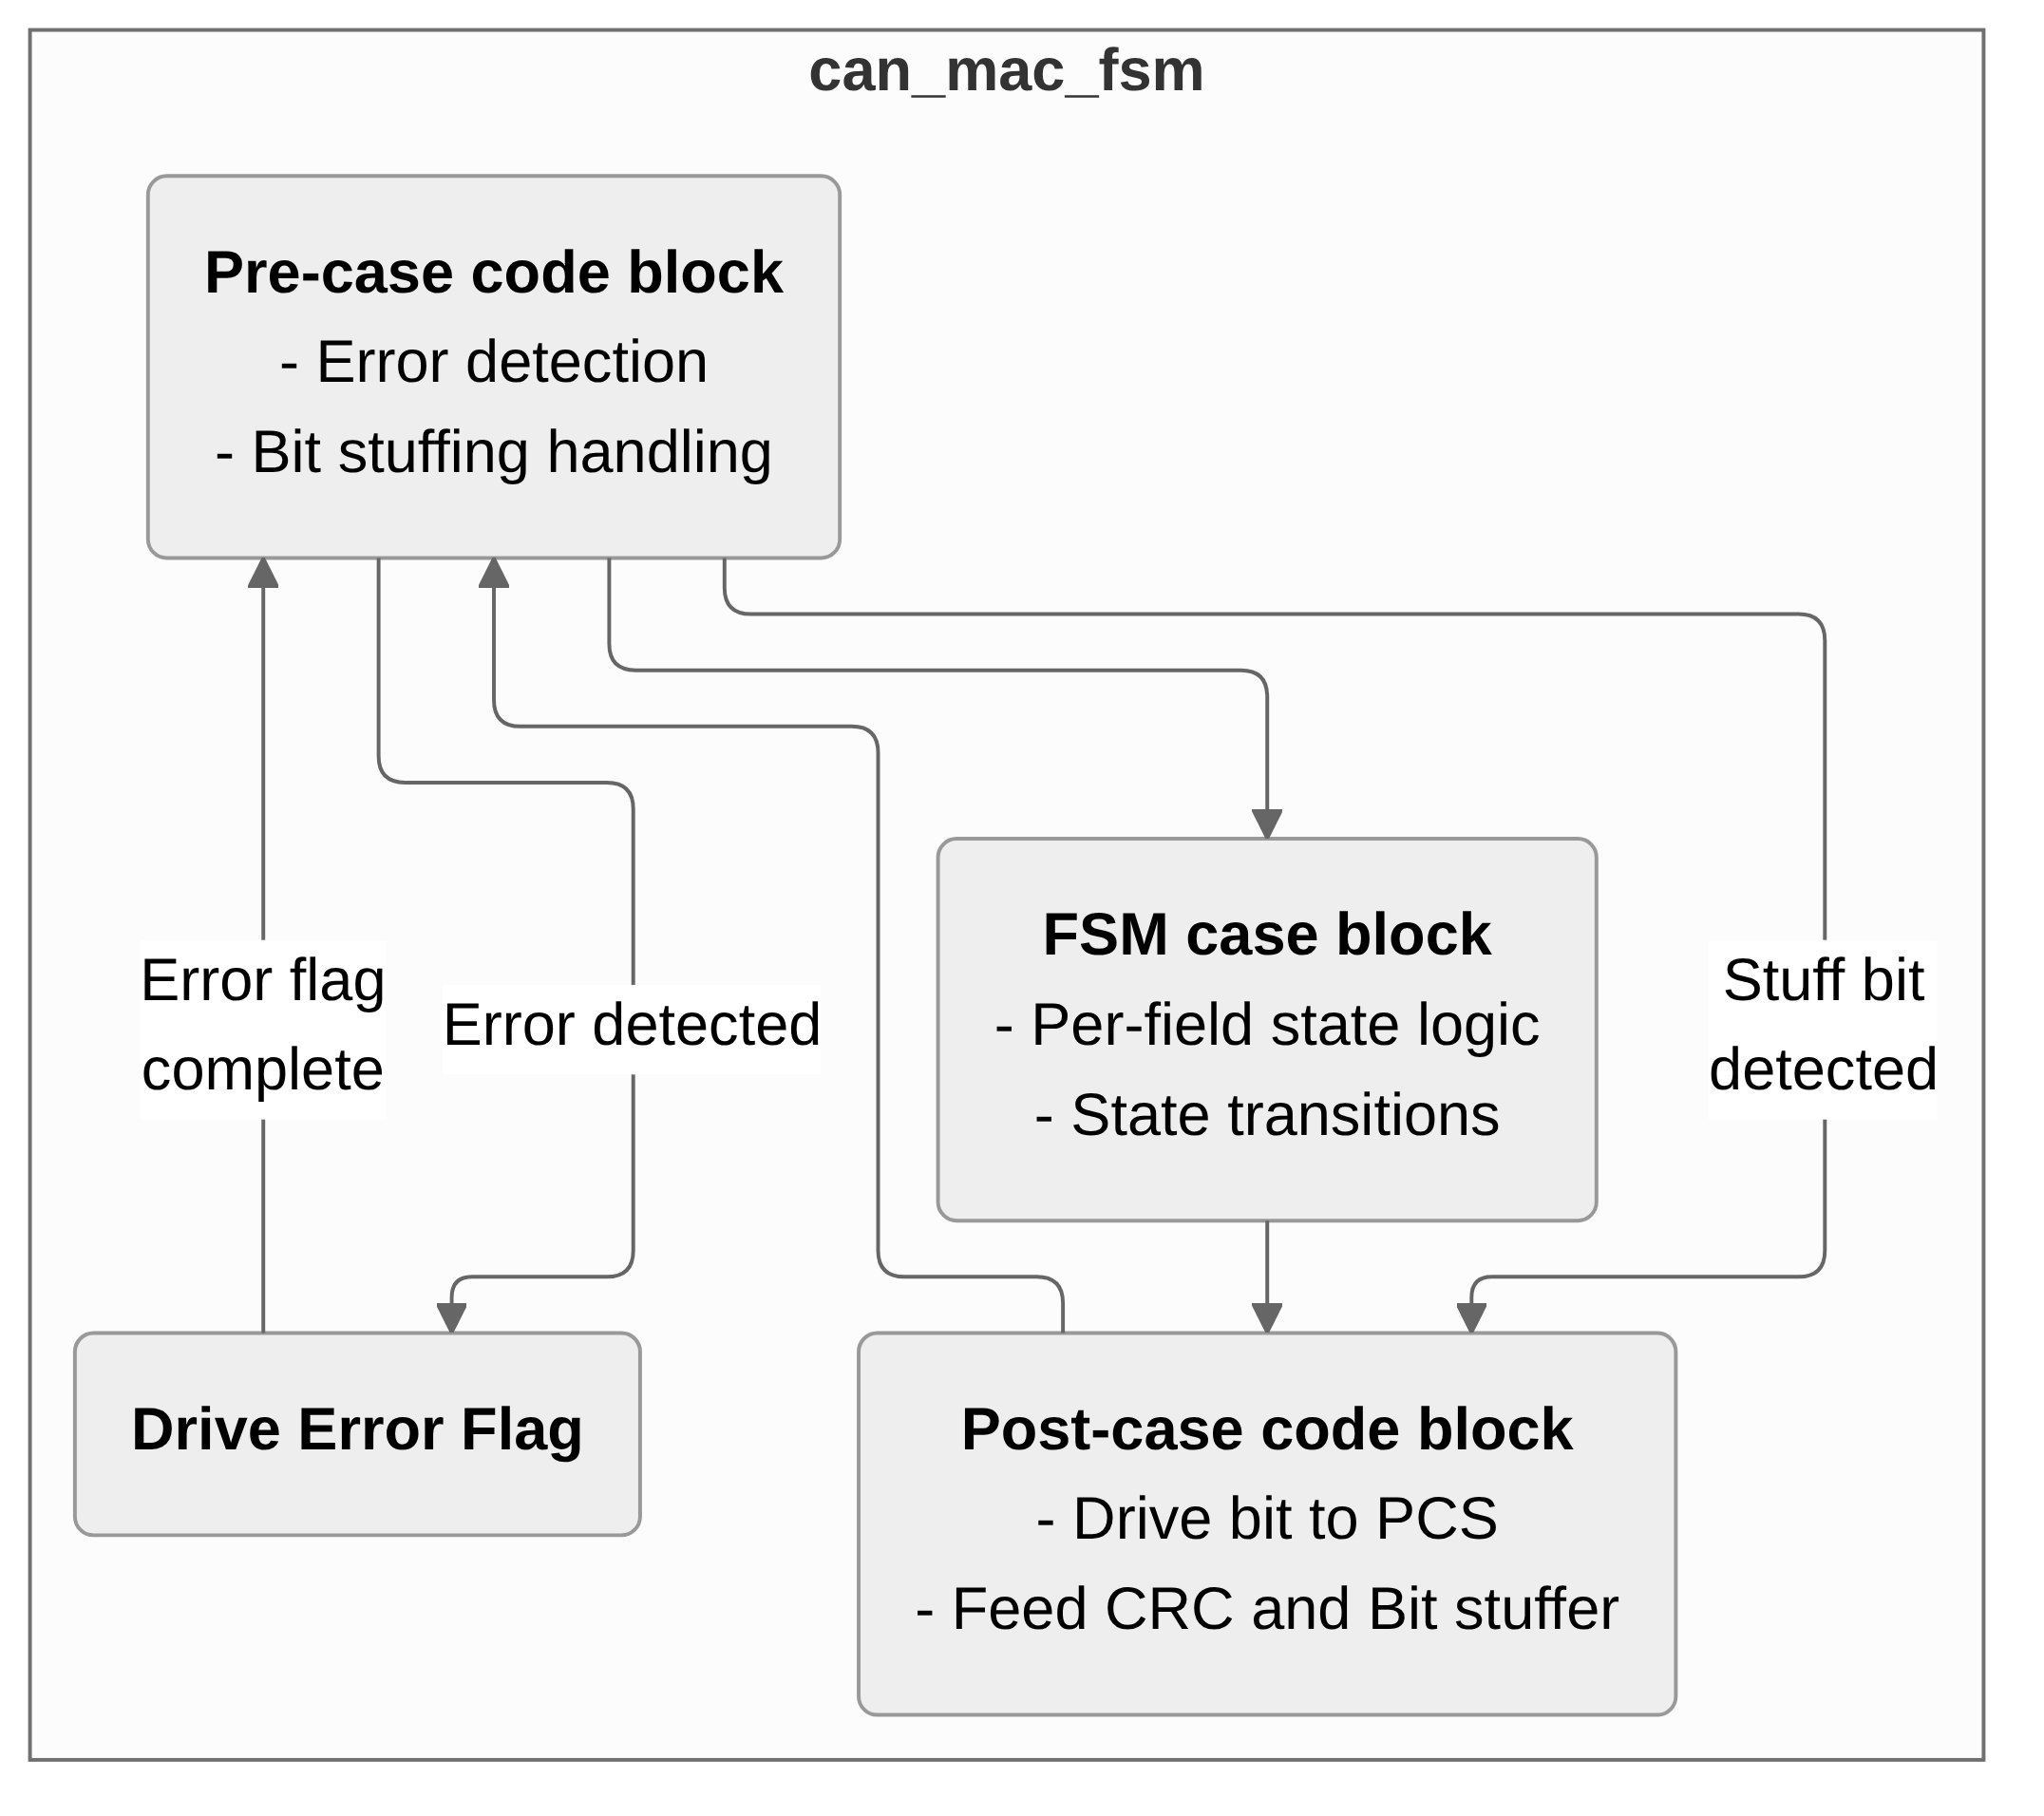
\includegraphics[,height=0.85\textheight,keepaspectratio]{images/fsm.png}
			\end{center}
		\end{column}
	\end{columns}
\end{frame}
\note{\footnotesize\begin{itemize}
		\item This slide covers \texttt{can\_mac\_fsm}. This \textbf{central orchestrator} of the MAC layer and is by far the largest module in the design. It relies on three peripheral helper modules handling bit stuffing, CRC, and TX serialization.
		\item \textbf{State graph:} CAN Classic and CAN FD are identical up to the FDF bit. From there the field sequences diverge --- BRS, ESI, longer data, SBC, different CRC. Each frame field is one FSM state. This makes the FSM directly readable against the frame structure, and the mapping from requirements to states clear.
		\item \textbf{\texttt{is\_transmitter}:} The FSM handles both TX and RX in a single state graph, with the \texttt{is\_transmitter} flag gating TX vs.\ RX logic within each state.
		\item \textbf{State transitions:} The FSM advances on the \textbf{sample point strobe} from \texttt{can\_pcs}. The next bit is then driven to \texttt{can\_pcs} two clock cycles later once \texttt{can\_mac\_bs} and \texttt{can\_mac\_crc} outputs have settled.
		\item \textbf{Streaming:} Valid received frames are streamed to LLC via a separate \textbf{Avalon-ST} interface control process.
	\end{itemize}}

% ==========================================
% SLIDE MAC-2: Bit stuffing
% ==========================================
\begin{frame}{MAC: \texttt{can\_mac\_bs} -- Bit Stuffing and Destuffing}
	\begin{columns}[c]
		\begin{column}{0.50\textwidth}
			\textbf{Dynamic stuffing} (CC and CF):
			\begin{itemize}\setlength{\itemsep}{6pt}
				\item Transmitter inserts inverse bit after five consecutive identical bits
				\item Receiver strips stuff bits and checks for violations
			\end{itemize}
			\vspace{0.4em}
			\textbf{Fixed stuffing} (CF CRC region only):
			\begin{itemize}\setlength{\itemsep}{6pt}
				\item Stuff bit at fixed intervals
				\item SBC: Gray-coded dynamic stuff count + parity
			\end{itemize}
		\end{column}
		\begin{column}{0.50\textwidth}
			\begin{center}
				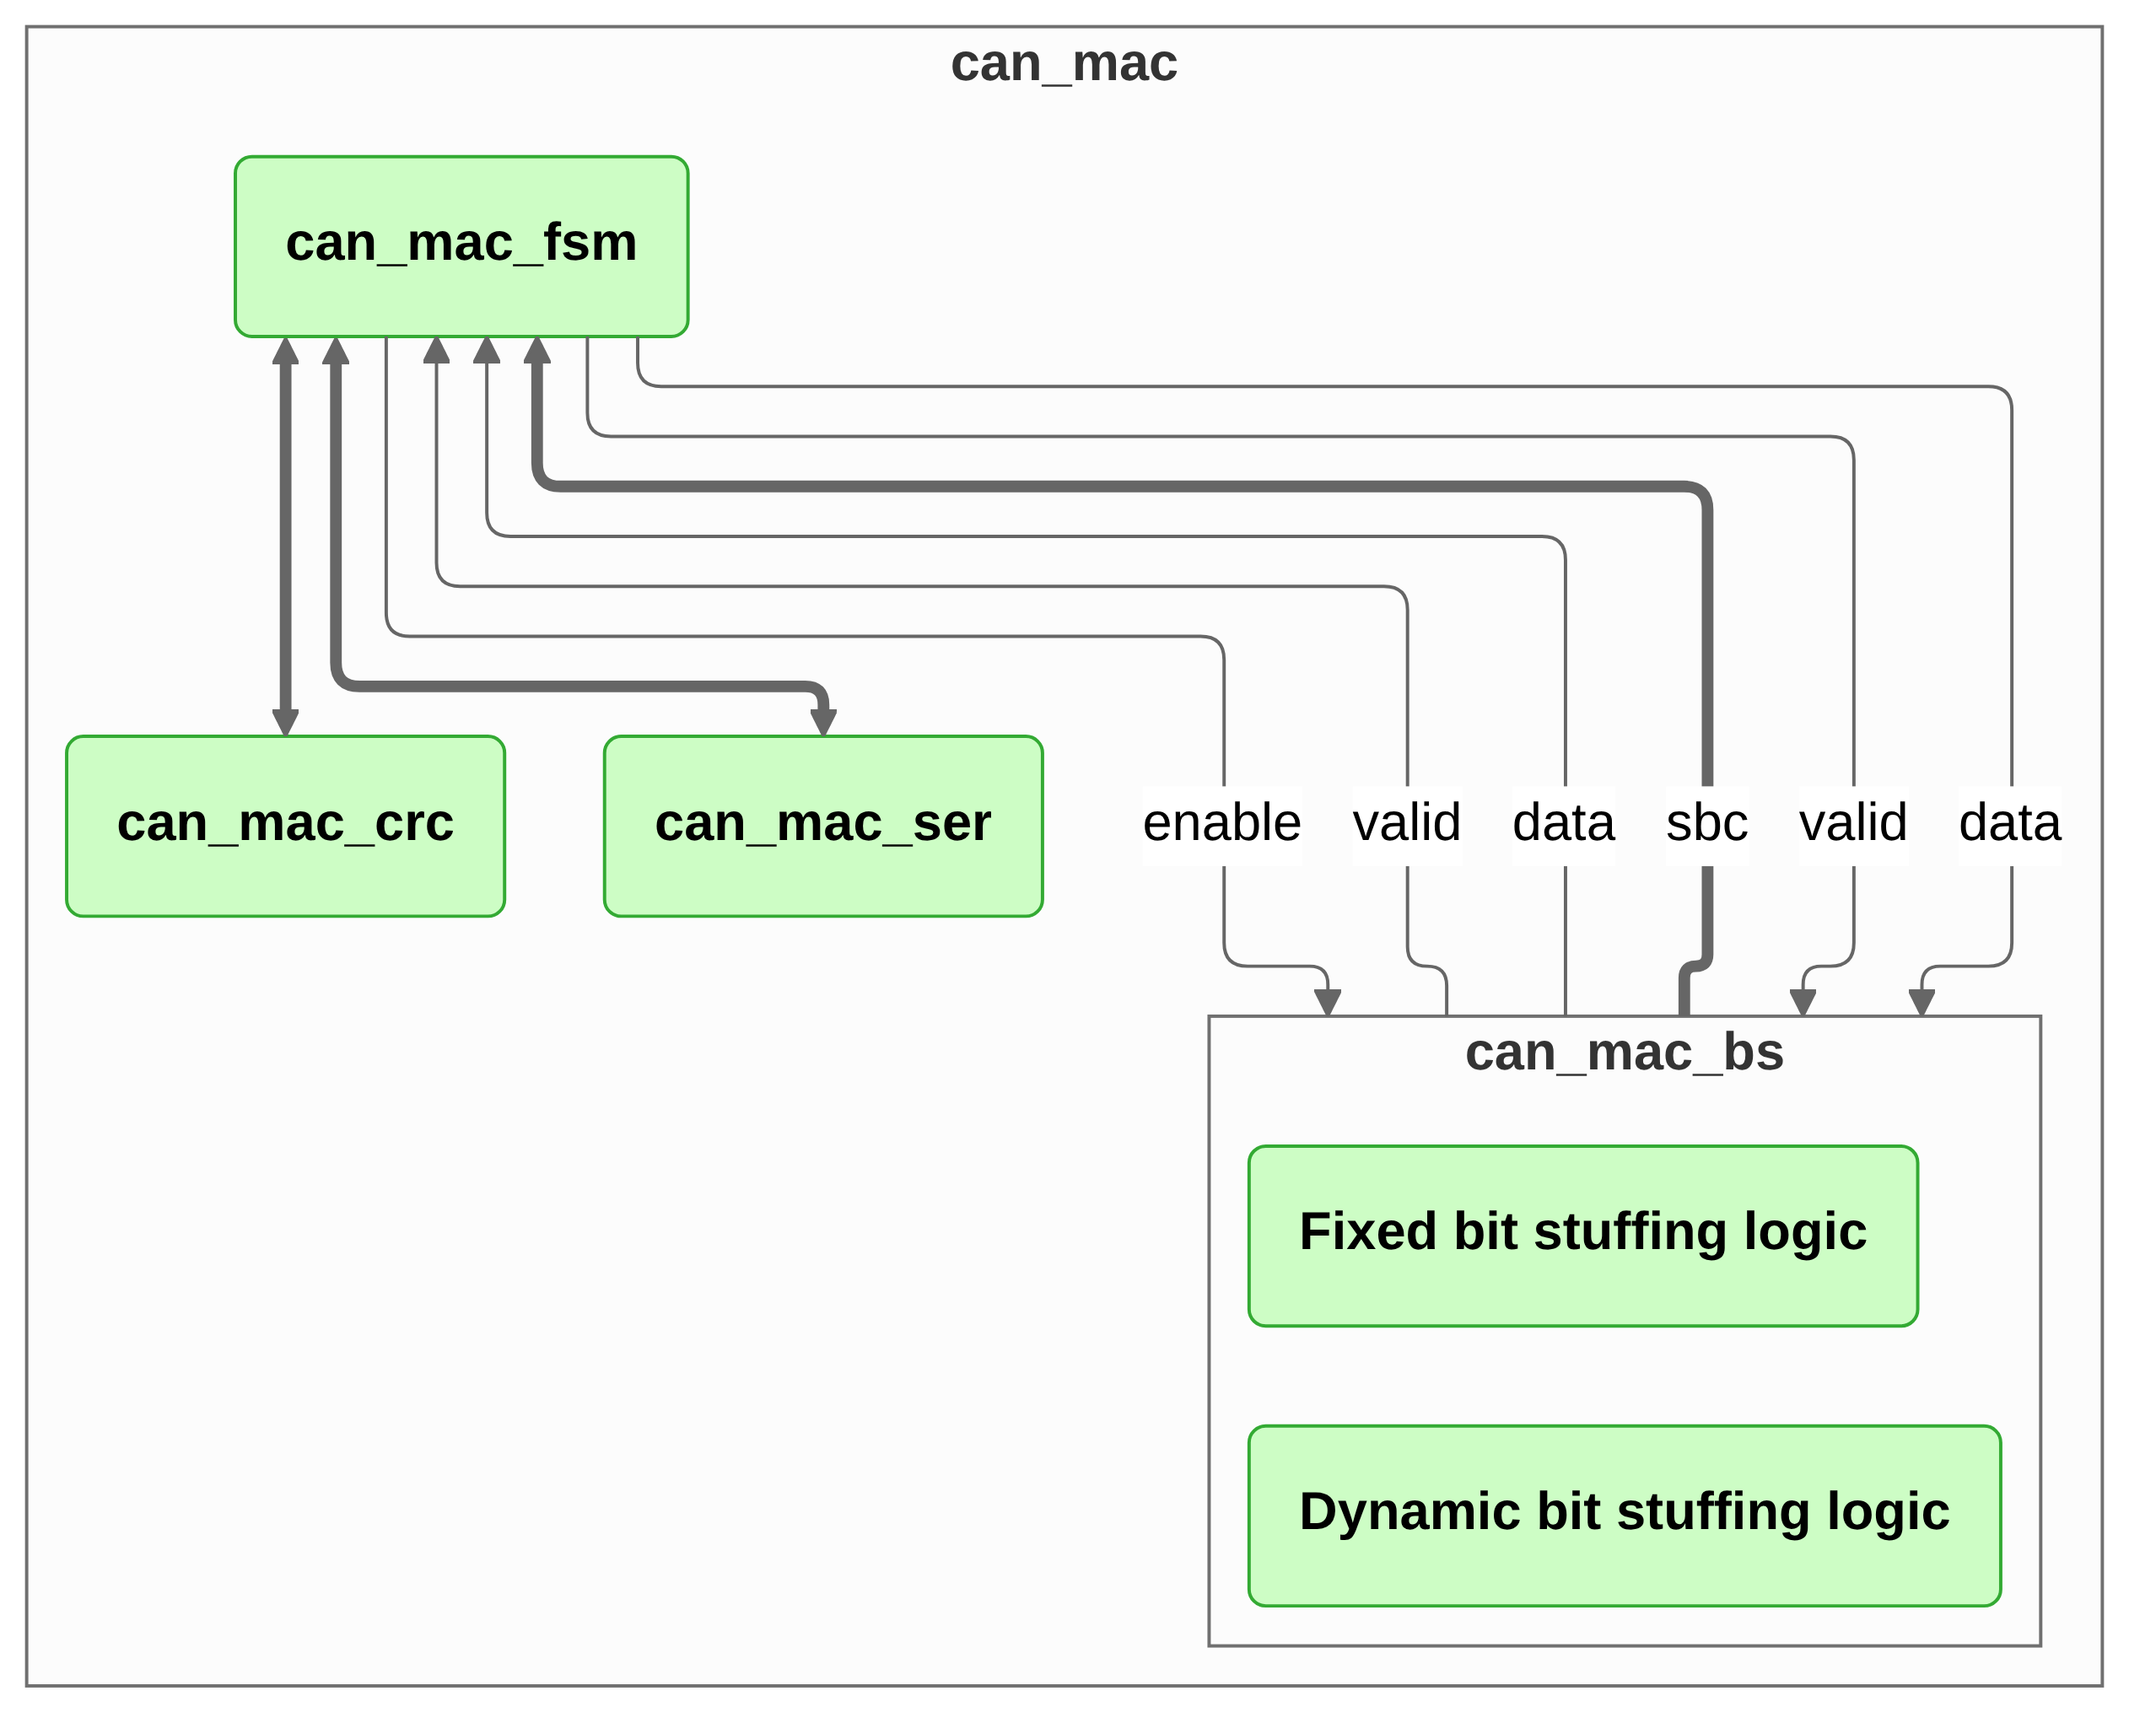
\includegraphics[width=1.0\textwidth,keepaspectratio]{images/bs.png}
			\end{center}
		\end{column}
	\end{columns}
\end{frame}
\note{\footnotesize\begin{itemize}
		\item This diagram shows the bit stuffing module and its interface with \texttt{can\_mac\_fsm}. It uses a two-way valid/data interface to and the enable signal selects dynamic vs. fixed bit stuffing. The SBC signal caries the 4-bit stuff bit count used in the CAN FD frame format.
		\item \textbf{Dynamic stuffing:} After five consecutive identical bits the transmitter inserts the inverse bit. The receiver strips it and flags a stuff error if the expected inverse bit is missing. Applies from SOF through the data field in both CC and CF.
		\item \textbf{Fixed stuffing:} In the CF CRC region, stuff bits are inserted at fixed intervals regardless of the data pattern --- not data-driven.
		\item \textbf{SBC:} Gray-coded count of dynamic stuff bits inserted since SOF, plus a parity bit. Transmitted before the CF CRC. This is the fix for the HD=2 problem --- any relocation of a dynamic stuff bit changes the SBC and therefore the CRC remainder.
	\end{itemize}}

% ==========================================
% SLIDE MAC-3: CRC
% ==========================================
\begin{frame}{MAC: \texttt{can\_mac\_crc} -- CRC Engine}
	\begin{columns}[c]
		\begin{column}{0.50\textwidth}
			\textbf{Three parallel engines}:
			\begin{itemize}\setlength{\itemsep}{6pt}
				\item CRC-15: CC frames
				\item CRC-17: CF frames, data payload $\leq$ 16\,bytes
				\item CRC-21: CF frames, data payload $>$ 16\,bytes
			\end{itemize}
			\vspace{0.4em}
			\textbf{Dual data feed}:
			\begin{itemize}\setlength{\itemsep}{6pt}
				\item \texttt{data\_cc}: de-stuffed stream
				\item \texttt{data\_fd}: includes dynamic stuff bits
			\end{itemize}
		\end{column}
		\begin{column}{0.50\textwidth}
			\begin{center}
				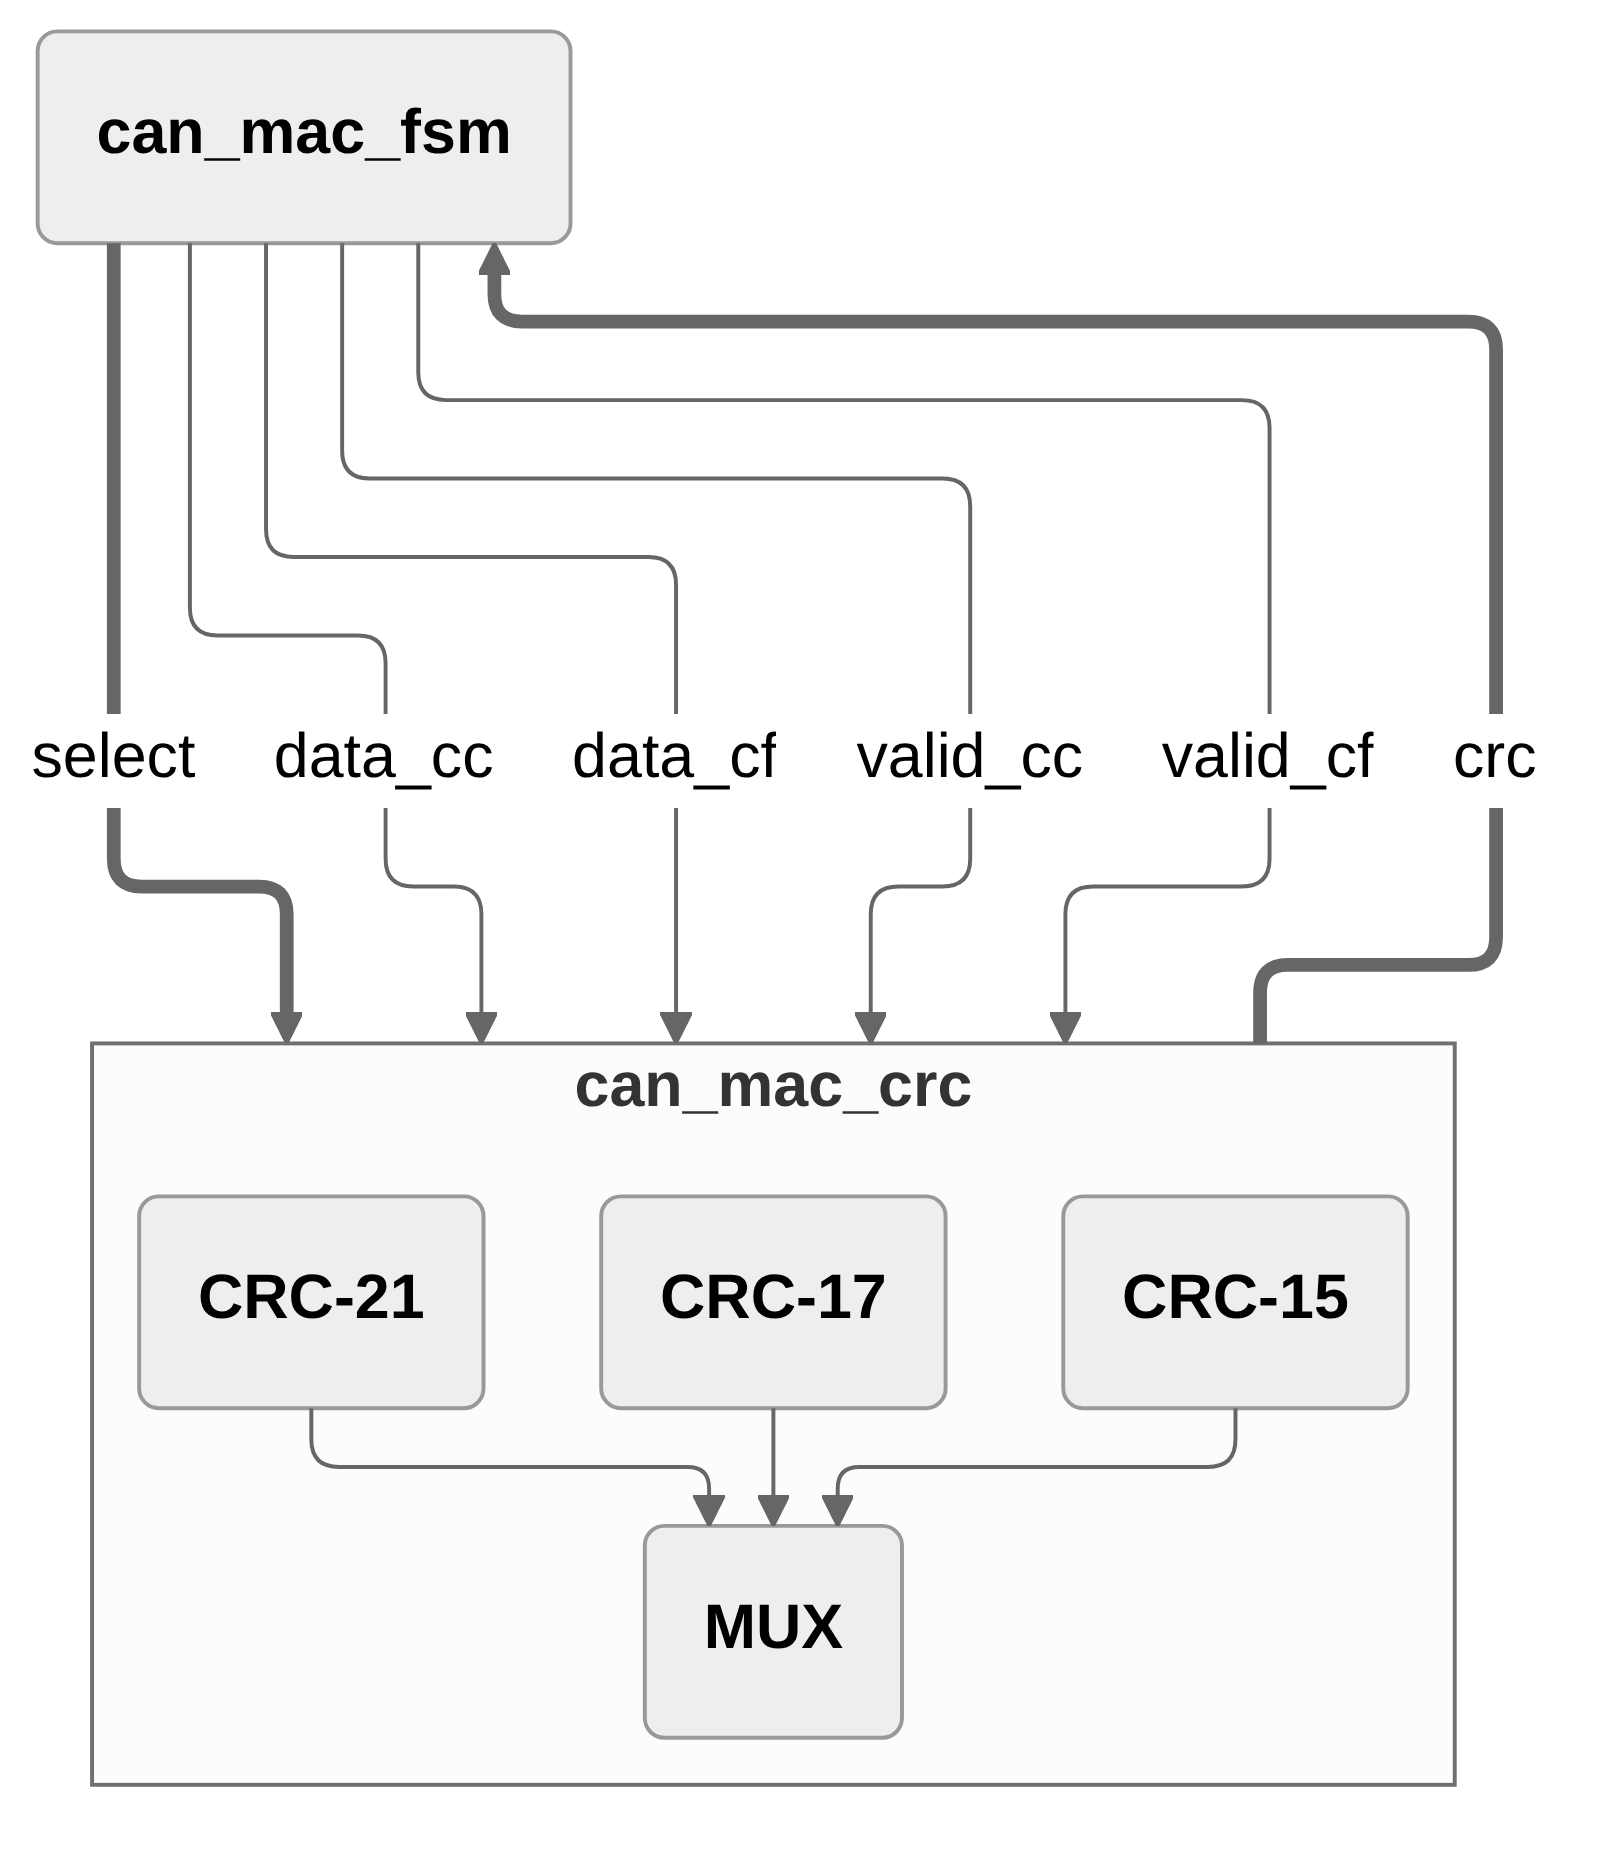
\includegraphics[width=1.0\textwidth,keepaspectratio]{images/crc.png}
			\end{center}
		\end{column}
	\end{columns}
\end{frame}
\note{\footnotesize\begin{itemize}
		\item And here we see the next MAC layer helper module (\texttt{can\_mac\_crc}) and its interface with \texttt{can\_mac\_fsm}. It runs \textbf{three CRC engines in parallel} -- one for each generator polynomial. It has a dual data feed from can\_mac\_fsm -- one for each frame format. The crc output signal is continuously updated and caries the result of the CRC calculation. The select input signal controls which CRC engine is routed to the output.
		\item \textbf{Three parallel engines:} CRC-15 for CC, CRC-17 for short CF payloads ($\leq$16 bytes), CRC-21 for longer CF payloads. Running in parallel avoids any timing dependency on knowing the format early.
		\item \textbf{Dual data feed:} \texttt{data\_cc} is the de-stuffed stream --- what CC receivers reconstruct. \texttt{data\_fd} includes dynamic stuff bits. CRC-17 and CRC-21 consume \texttt{data\_fd}. The dual feed is needed since receivers don't know the frame format until after the DLC field.
	\end{itemize}}

% ==========================================
% SLIDE MAC-4: Serializer
% ==========================================
\begin{frame}{MAC: \texttt{can\_mac\_ser} -- TX Frame Serializer}
	\begin{columns}[c]
		\begin{column}{0.70\textwidth}
			\begin{itemize}
				\item Converts LLC byte stream to serial bit stream for \texttt{can\_mac\_fsm}
				\item Receives frame from LLC over Avalon-ST interface
				\item Extracts frame metadata (IDE, FDF, DLC, FTYP, BRS, ESI) from two leading config bytes in LLC frame
			\end{itemize}
		\end{column}
		\begin{column}{0.30\textwidth}
			\begin{center}
				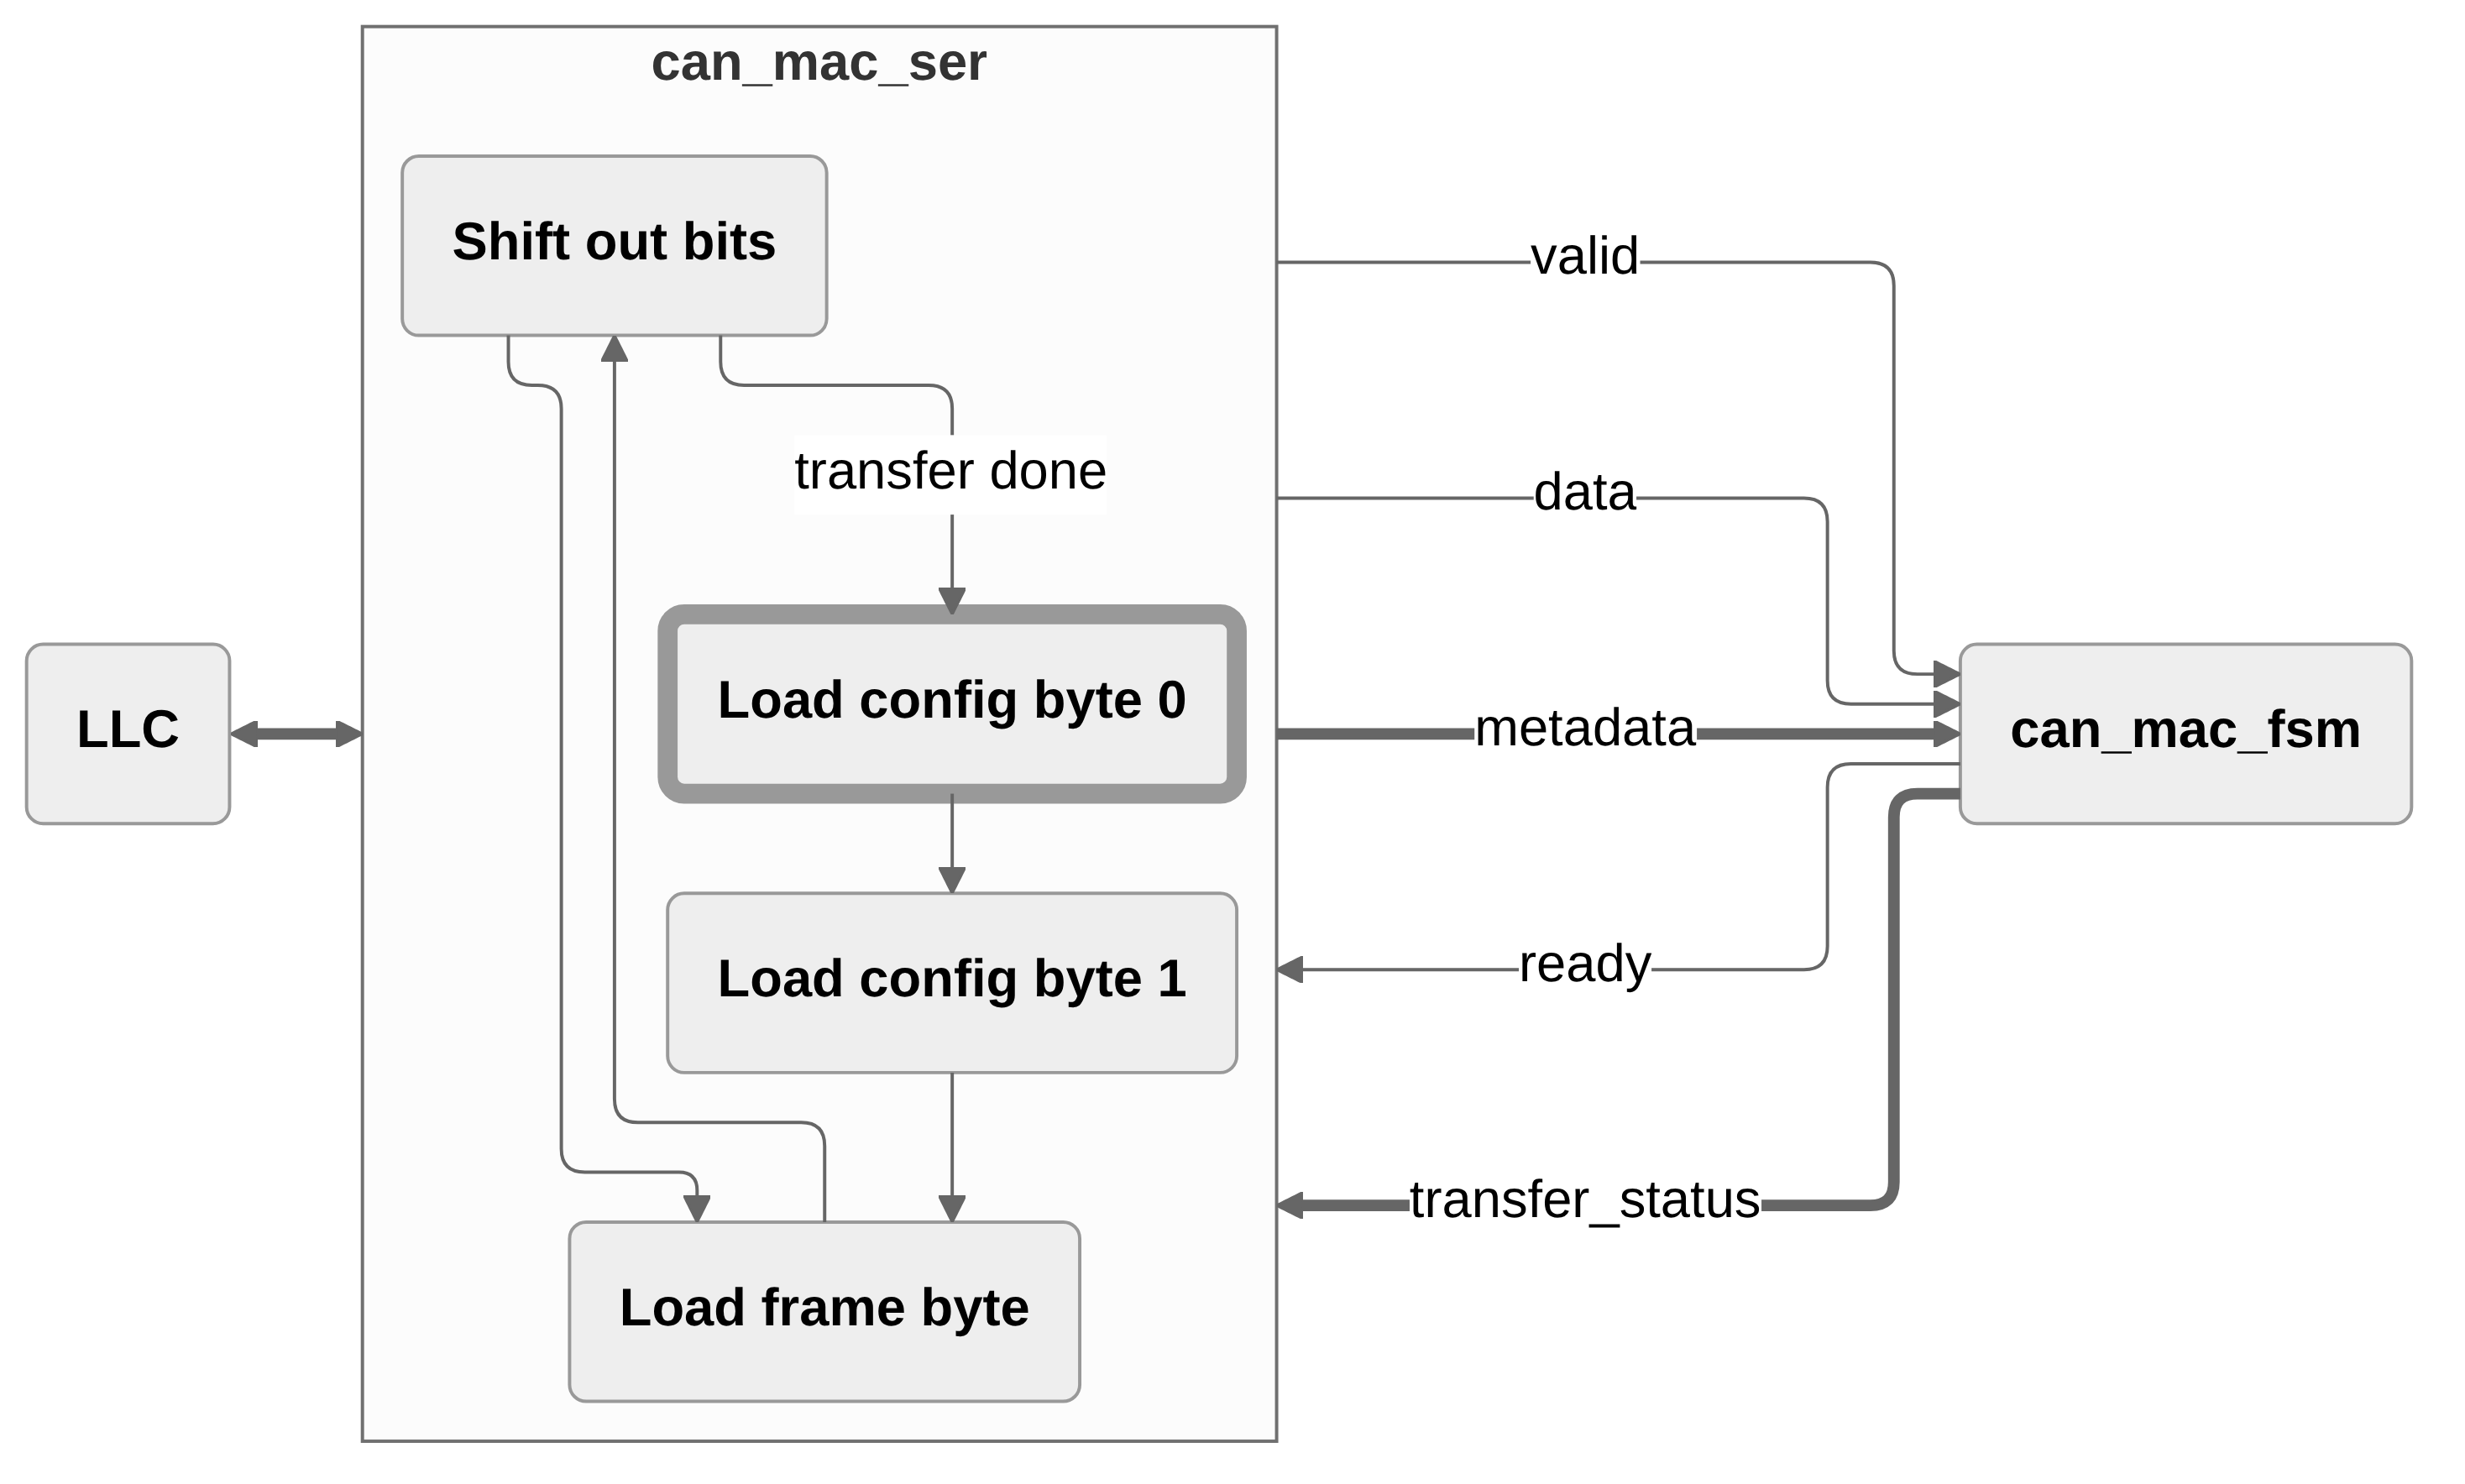
\includegraphics[height=0.90\textheight,keepaspectratio]{images/ser.png}
			\end{center}
		\end{column}
	\end{columns}
\end{frame}
\note{\footnotesize\begin{itemize}\setlength{\itemsep}{5pt}
		\item And this diagram shows the FSM of the last of the mac layer helper modules - the TX frame serializer along with its interface with \texttt{can\_mac\_fsm}. The modules interfaces with the LLC through an Avalon-ST interface and the serialised stream is transferred to \texttt{can\_mac\_fsm} using a ready/valid handshake.
		\item \textbf{LLC byte stream to serial bit stream:} The LLC-frame front-loads all metadata into two leading config bytes, and \texttt{can\_mac\_ser} can begin streaming ID and data bits after receiving these.
		\item \textbf{Metadata extraction:} The metadata contained in the config bytes (IDE, FDF, DLC, FTYP, BRS, and ESI) are presented on the metadata signal and held stable for the duration of frame transmission - guiding the format selection logic of can\_mac\_fsm.
		\item \textbf{Transfer status:} The \texttt{transfer\_status} signal caries the status of the latest attempted transmission. It is used to reset the FSM and forwarded back to the LLC.
	\end{itemize}}

% ==========================================
% SLIDE MAC-5: FCE
% ==========================================
\begin{frame}{FCE: \texttt{can\_fce} -- Fault Confinement Entity}
	\begin{itemize}\setlength{\itemsep}{10pt}
		\item The error counting FSM has three states: error active, error passive, bus off -- driven by TEC and REC thresholds.
		\item The module subscribes to error events from \texttt{can\_mac\_fsm}. It signals \texttt{error\_active} and \texttt{bus\_off} back according to the thresholds of the error counting FSM.
		\item An active bus-off signal is lowered after 128 \texttt{idle\_condition} strobes from \texttt{can\_pcs}
	\end{itemize}
\end{frame}
\note{\footnotesize\begin{itemize}
		\item The FCE requirements are implemented in the \texttt{can\_fce} module. The module sits outside the data path and monitors TX and RX error events. It maintains error counters and updates the node error state accordingly.
		\item \textbf{Three states:} TEC and REC are incremented by 8 on errors and decremented by 1 on success. Above 127 the node enters \textbf{error passive} --- its error flags are recessive and invisible to other nodes. Above 255 it goes \textbf{bus off} and stops driving entirely.
		\item \textbf{Error events:} \texttt{can\_mac\_fsm} signals error events to FCE --- including \texttt{passive\_tx\_ack\_error} (ISO exempts this from TEC increment to avoid stranding an error-passive transmitter at bus off) and \texttt{error\_delim\_to\_late} (stuck-dominant fault, hits both counters by 8).
		\item \textbf{Bus-off recovery:} ISO mandates 128 sequences of 11 recessive bits --- an extended quiet period before re-joining. The \texttt{idle\_condition} strobe from \texttt{can\_pcs} counts these.
	\end{itemize}}

% ==========================================
% SLIDE: TDC concept
% ==========================================
\begin{frame}{Transmitter Delay Compensation (TDC)}
	\begin{center}
		
\includegraphics[width=\textwidth,keepaspectratio]{\figures/tdc.png}
	\end{center}
	\begin{itemize}
		\item At high data rates the \textbf{transceiver loop delay} can exceed the bit time -- TX echo arrives too late for the normal SP
		\item Without compensation \textbf{bit-error monitoring} fails in the data phase
		\item TDC measures the delay on the \textbf{reserved bit} and defers the \textbf{SSP} to match
	\end{itemize}
\end{frame}
\note{\footnotesize\begin{itemize}\setlength{\itemsep}{5pt}
		\item Before describing the PCS module I want to take a brief detour to explain Transmitter Delay Compensation \textbf{TDC} -- it is the key concept driving the additional complexity bit-timing in CAN FD frame transmission.
		\item \textbf{The problem:} The transmitter detects bit errors by monitoring its own echo on the bus. At high data rates the transceiver loop delay can exceed the bit period --- the echo arrives too late. If the transmitter uses the normal SP it reads the previous bit, not the one it just drove --- so bit errors go undetected and fault confinement breaks down.
		\item \textbf{Invalid SSP:} The figure shows TX driving bits and the delayed RX echo. The SP fires at the wrong position during the early data-phase bits --- marked "Invalid SSP" --- because the echo has not yet arrived. Once the TDC offset is known the SSP fires correctly, aligned with the actual echo.
		\item \textbf{TDC measurement:} The transmitter drives the \textbf{FDF bit} and starts a counter. It watches for the RX echo of the \textbf{reserved bit}. The counter value when the echo arrives is the \textbf{transmitter delay} --- this offset is then applied to every subsequent SSP in the data phase.
	\end{itemize}}

% ==========================================
% SLIDE 6: PCS
% ==========================================
\begin{frame}{PCS: \texttt{can\_pcs} -- Bit Timing and Transmitter Delay Compensation (TDC)}
	\begin{columns}[c]
		\begin{column}{0.50\textwidth}
			\begin{itemize}\setlength{\itemsep}{6pt}
				\item SP strobes at end of PHASE\_SEG1
				\item Transmit bit on TX line at end of PHASE\_SEG2
				\item SSP strobe used for bit-error monitoring in data phase
				\item Switch to data phase bit rate at BRS bit
				\item Transceiver loop delay measured on res bit
			\end{itemize}
		\end{column}
		\begin{column}{0.50\textwidth}
			\begin{center}
				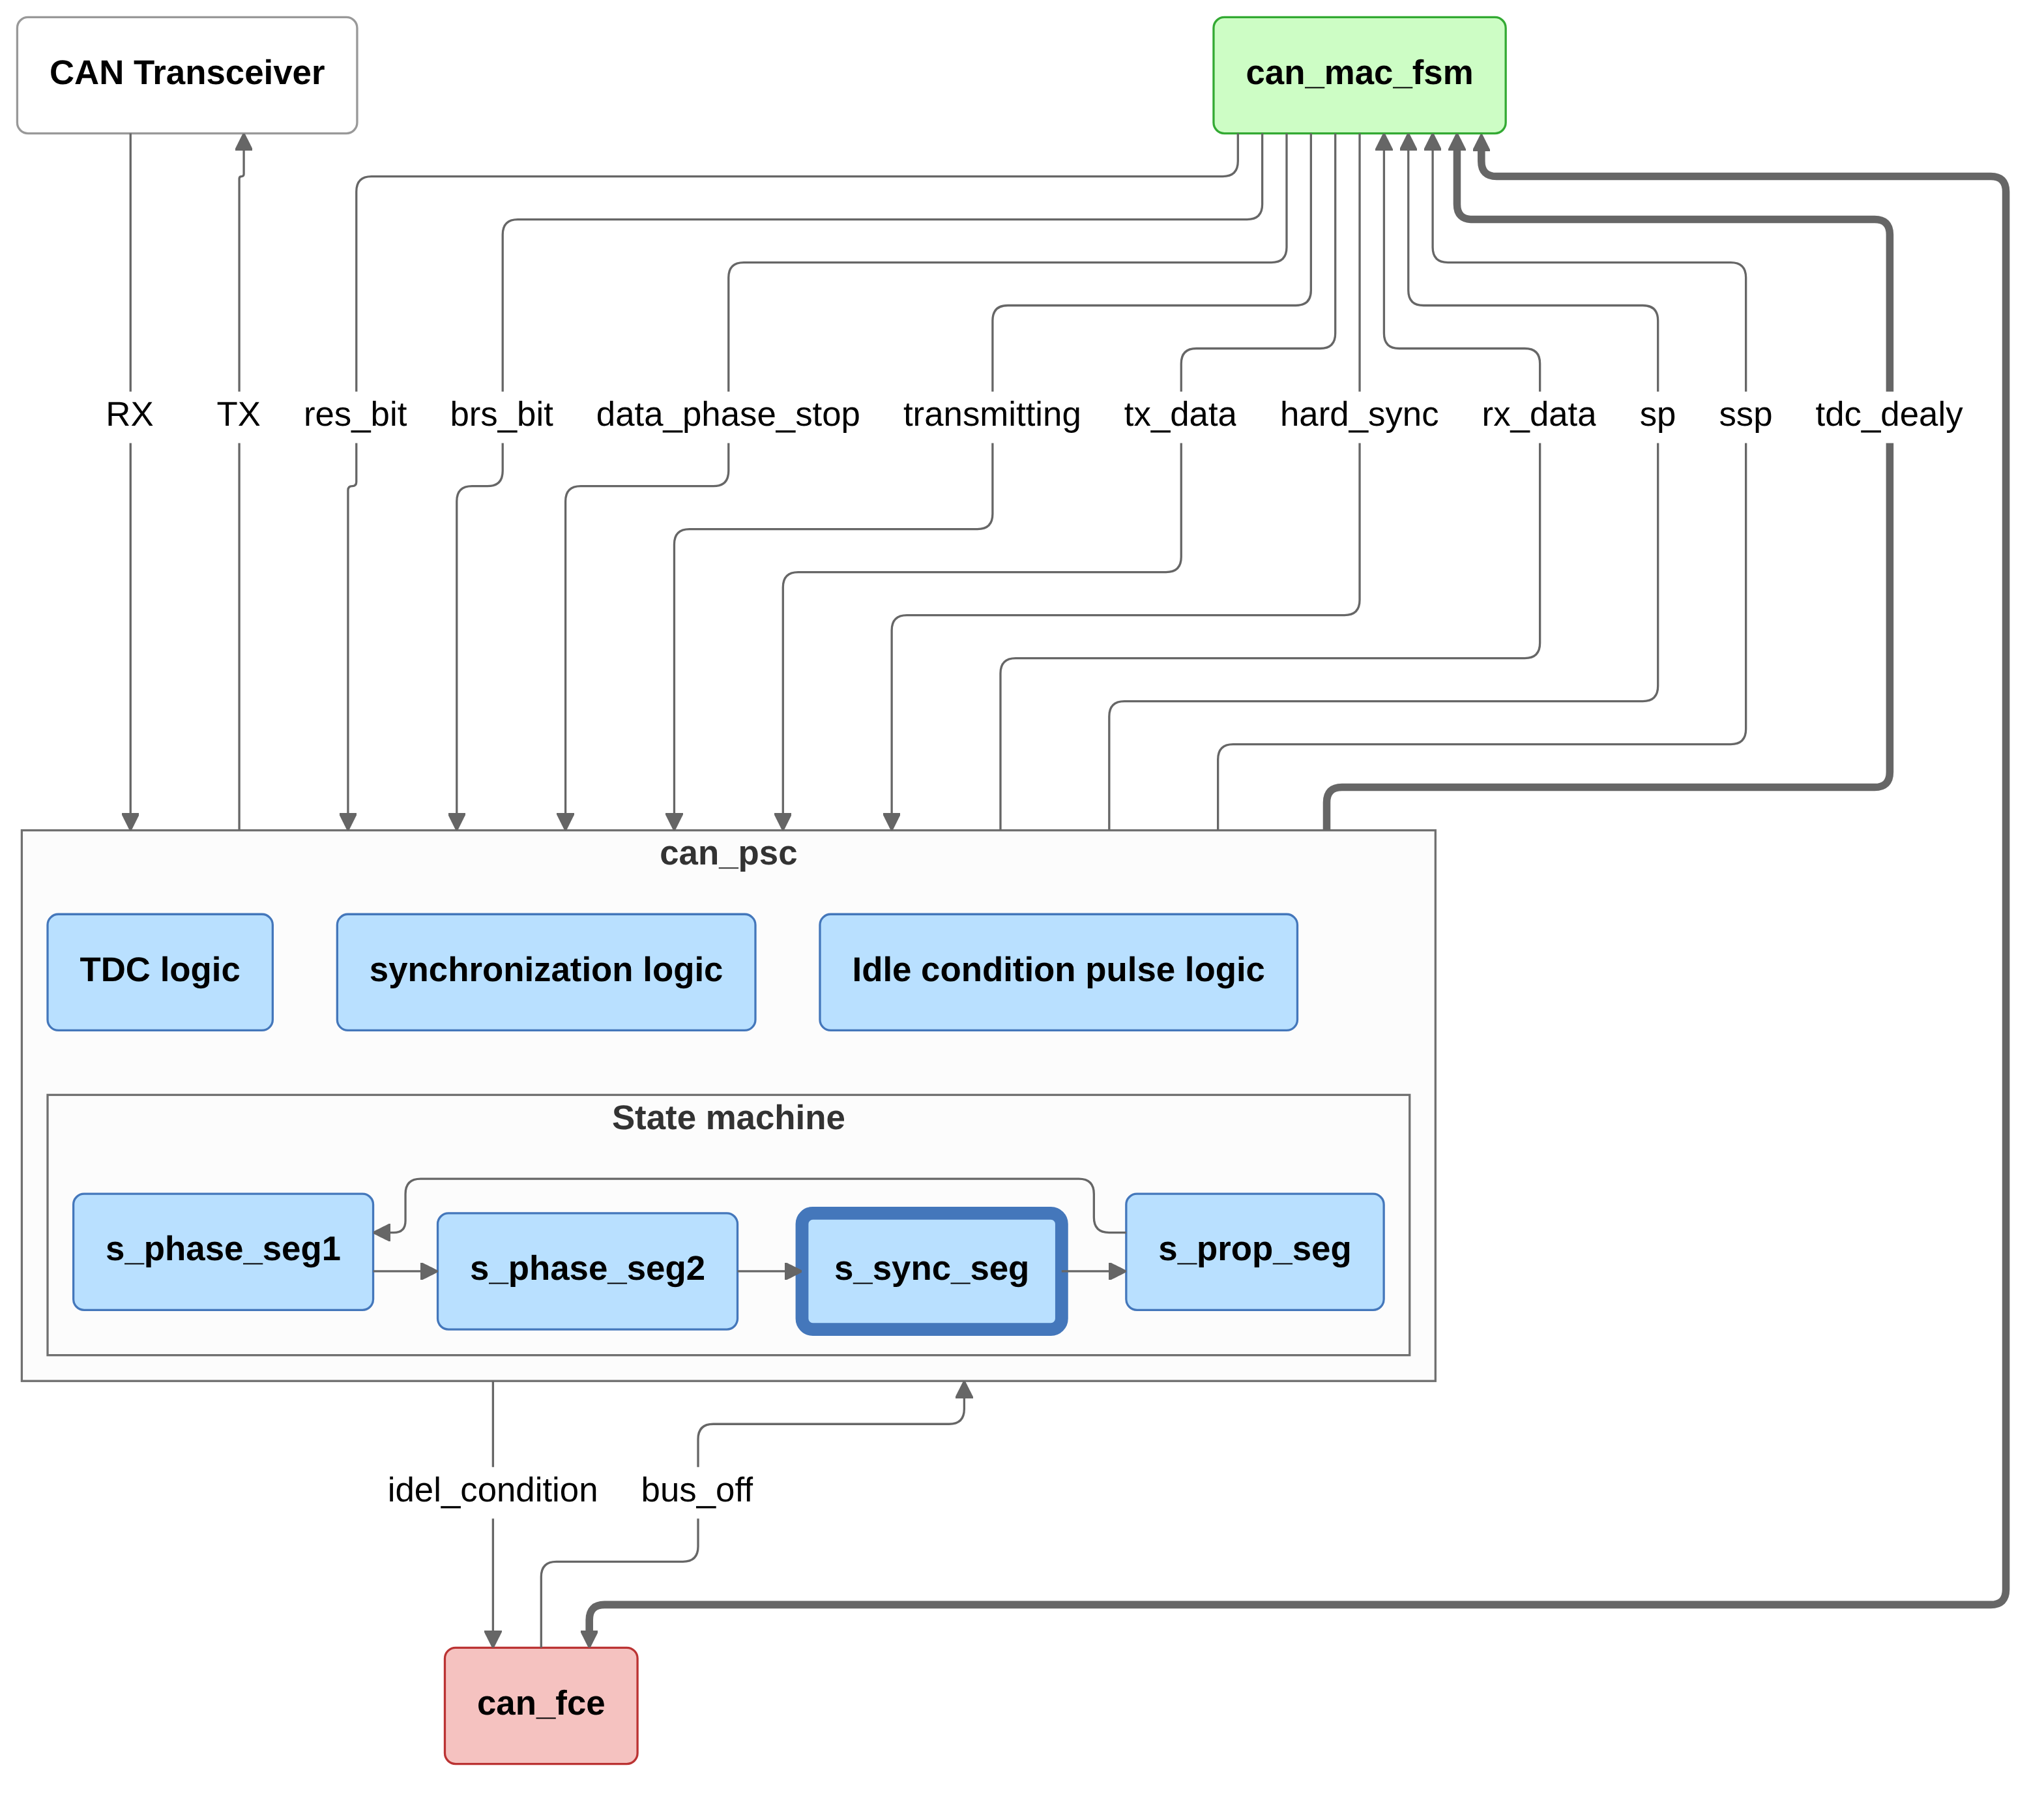
\includegraphics[width=\textwidth,height=0.75\textheight,keepaspectratio]{images/pcs.png}\\[0.3em]
			\end{center}
		\end{column}
	\end{columns}
\end{frame}
\note{\footnotesize\begin{itemize}
		\item Great -- now that TDC is clear, let's look at the \textbf{PCS implementation}. The diagram shows \texttt{can\_pcs} and its interface with \texttt{can\_mac\_fsm}. The PCS generates \textbf{sp} and \textbf{ssp} strobes that MAC FSM use for state transition and data-phase bit-error error monitoring.
		\item \textbf{Interface:} \texttt{can\_mac\_fsm} drives \textbf{brs\_bit}, \textbf{res\_bit}, and \textbf{data\_phase\_stop} into the PCS --- these are exactly the signals the TDC logic needs. \textbf{brs\_bit} triggers the rate switch, \textbf{res\_bit} triggers the TDC measurement, \textbf{data\_phase\_stop} signals the return to nominal rate. The PCS outputs \textbf{sp}, \textbf{ssp}, and \textbf{tdc\_delay} back to the MAC FSM. The MAC FSM maintains a fifo of transmitted bits and the \textbf{tdc\_delay} is used to select the relevant bit for error detection. The module also generates the idel\_condition strobe during bus-off used by FCE for bus-off recovery.
		\item The \textbf{SP strobe} is controlled by the main PCS FSM and fires at the end of Phase\_Seg1. Hard sync is initiated my the MC FSM through the hard\_sync signal and resync adjusts Phase\_Seg1 or Phase\_Seg2 mid-frame.
	\end{itemize}}

% ==========================================
% SLIDE 8: Bus-off recovery
% ==========================================
\section{Verification}
% ==========================================
% SLIDE 9a: Verification plan methodology
% ==========================================
\begin{frame}{Verification Plan}
	\begin{columns}[c]
		\begin{column}{0.42\textwidth}
			\begin{itemize}\setlength{\itemsep}{8pt}
				\item Each requirement augmented with verification fields
				\item MCP server enforces typed writes --- agents update status, labels, and file links safely throughout the project
				\item Traceability: \texttt{label} names the TB procedure; \texttt{file} points to the testbench
			\end{itemize}
		\end{column}
		\begin{column}{0.58\textwidth}
			\footnotesize
			\renewcommand{\arraystretch}{1.4}
			\begin{tabular}{>{\ttfamily}l p{0.55\textwidth}}
				\toprule
				\multicolumn{2}{l}{\textit{(id, paraphrase, layer, priority from D\&I)}} \\
				\midrule
				side          & TX / RX / both                                           \\
				format        & CB / CE / FB / FE                                        \\
				observability & black\_box / white\_box                                  \\
				method        & simulation / waveform / inspection                       \\
				status        & not\_started / in\_progress / complete                   \\
				label         & TB procedure or RTL tag                                  \\
				file          & Testbench or RTL source file                             \\
				\bottomrule
			\end{tabular}
		\end{column}
	\end{columns}
\end{frame}
\note{\footnotesize\begin{itemize}\setlength{\itemsep}{5pt}
		\item That concludes design and implementation. Now  let's have a look at \textbf{verification}. Each requirement from the D\&I phase is augmented with a set of verification fields that track how and whether it is verified.
		\item \textbf{Each requirement augmented:} \textbf{side} (TX/RX/both), \textbf{format} (which frame formats apply), \textbf{observability} (black-box port-level or white-box waveform inspection), \textbf{method} (simulation, waveform, or RTL inspection), \textbf{status}, and \textbf{traceability} fields pointing to the TB procedure and file.
		\item \textbf{MCP server:} The requirements are stored in a TOML file. Direct AI edits to large structured files are error-prone --- the MCP server wraps it with a typed write interface so each update targets a single field and is schema-validated before it reaches the file.
		\item \textbf{Traceability:} \texttt{label} names the exact TB procedure that closes the requirement. \texttt{file} points to the testbench source. Every closed requirement has a direct link to its evidence.
	\end{itemize}}

% ==========================================
% SLIDE 9b: Verification results
% ==========================================
\begin{frame}{Verification Results -- 28 of 37 requirements closed}
	\begin{itemize}\setlength{\itemsep}{8pt}
		\item \textbf{Testbench coverage:} Unit TB per module and an integrated two-node bus simulation TB
		\item \textbf{LLC not implemented:} 6 LLC-related requirements \textbf{not started}. LLC adds acceptance filtering and retransmission on arbitration loss. MAC, PCS, and FCE are sufficient for full frame TX/RX.
		\item \textbf{2 not started:} Both \textbf{optional} and \textbf{non-blocking}. \textbf{REQ-034} applies to implementations buffering TX frames in MAC. This design uses direct streaming. \textbf{REQ-035} is error signalling enable/disable.
		\item \textbf{REQ-021 in progress:} Sub-claim~1 verified (Bit-error detection). Sub-claims 2-5 require frame-aware error injection into a running frame - not supported in the current test environment.
	\end{itemize}
\end{frame}
\note{\footnotesize\begin{itemize}\setlength{\itemsep}{5pt}
		\item \textbf{28 of 37 closed} means all P1 MAC, PCS, and FCE requirements are verified. The nine open items fall into three categories.
		\item \textbf{LLC not implemented:} Six LLC requirements not started --- deferred due to time constraints. The controller functions correctly without LLC as discussed earlier.
		\item \textbf{REQ-034 not applicable:} Conditional on using shared memory for MAC frames. This design streams directly via Avalon-ST --- the condition never applies.
		\item \textbf{REQ-021 in progress:} Sub-claim 1 (SP bit-error detection) is verified. Sub-claims 2--5 require injecting an error into a specific bit position within a running frame --- not supported by the current testbench environment.
	\end{itemize}}

% ==========================================
% SLIDE: Integration testbench
% ==========================================
\begin{frame}{Integration Testbench Architecture}
	\begin{center}
		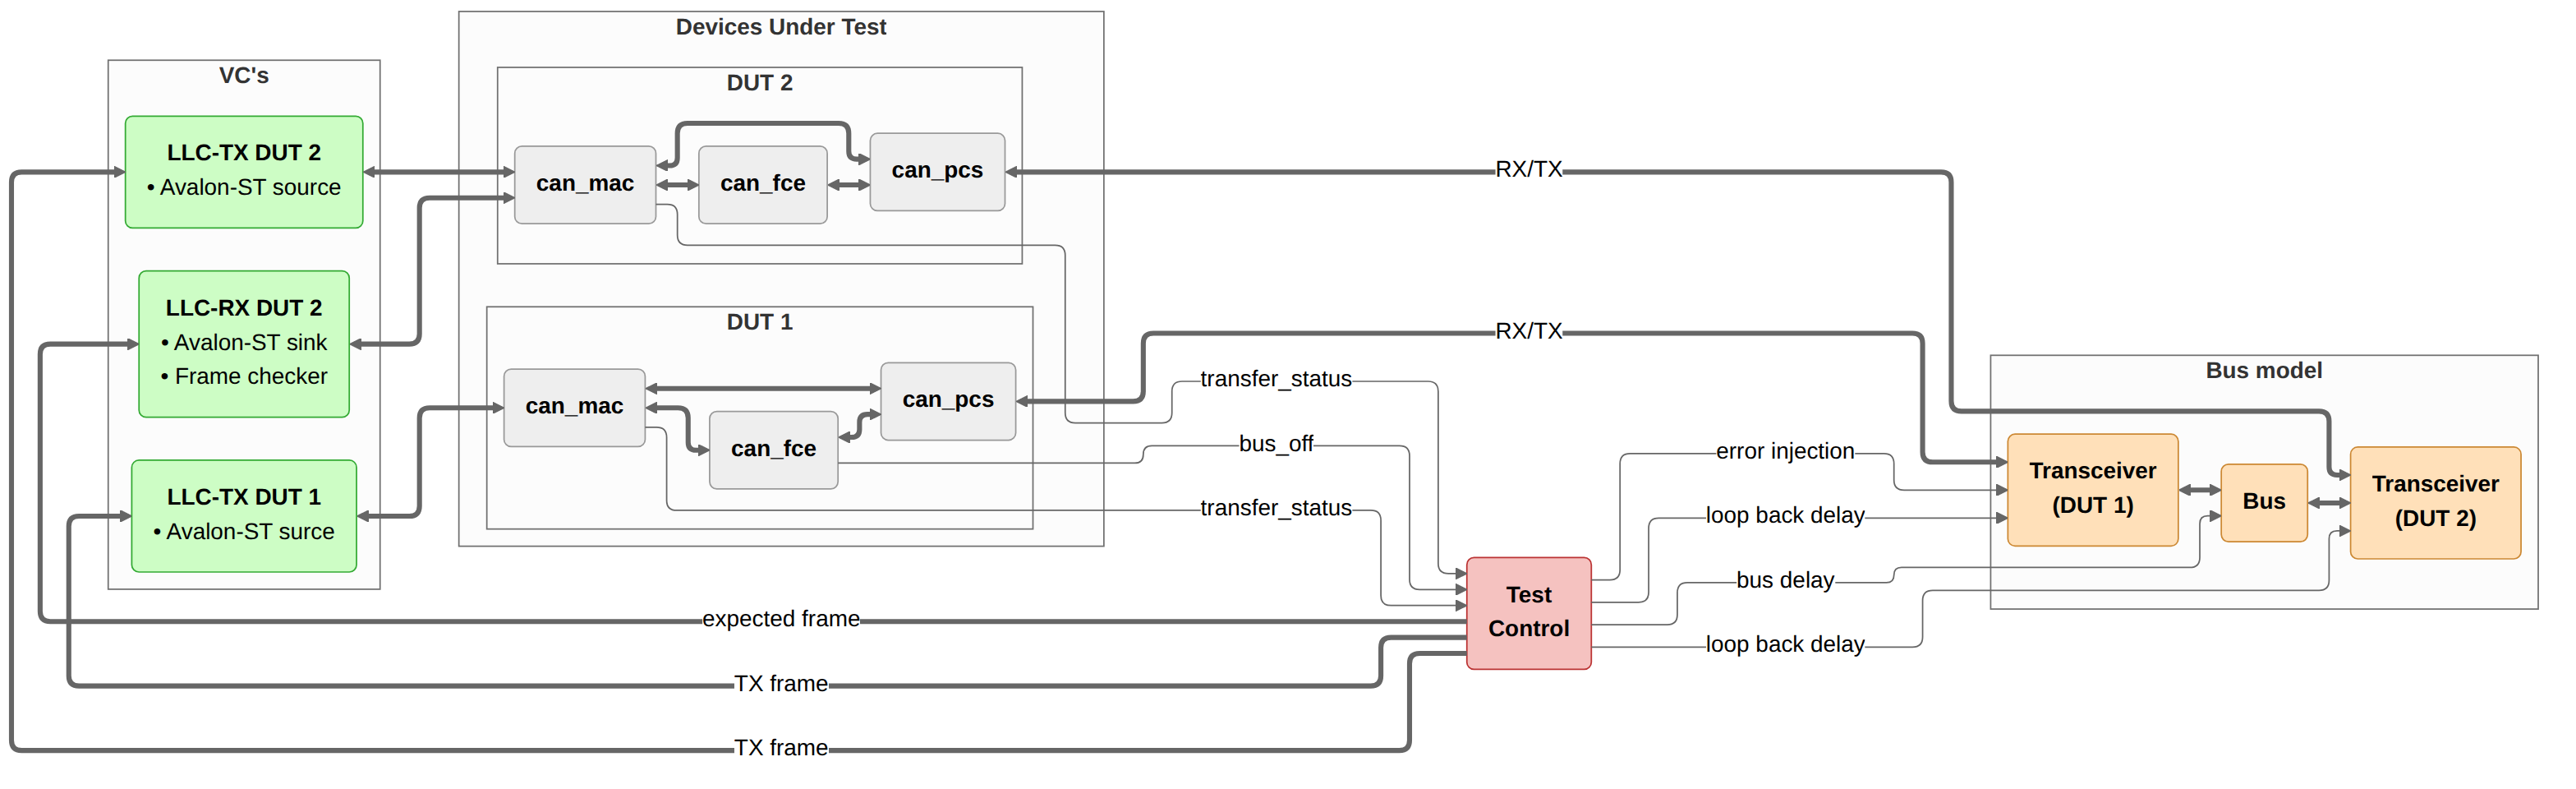
\includegraphics[width=\textwidth,height=0.62\textheight,keepaspectratio]{images/ver.png}
	\end{center}
	\vspace{0.2em}
	\footnotesize
	\begin{itemize}\setlength{\itemsep}{3pt}
		\item Two independent \texttt{can\_mac\_pcs\_fce} instances --- what DUT~1 transmits, DUT~2 must receive correctly and vice versa
		\item Bus model with configurable loop delay and error injection controlled by \texttt{p\_test\_ctrl}
		\item \texttt{rx\_llc\_dut\_2} checks received frames against expected frames from the TX source
	\end{itemize}
\end{frame}
\note{\footnotesize\begin{itemize}\setlength{\itemsep}{5pt}
		\item Each module has its own \textbf{unit testbench}. The integration TB shown here puts two full controller instances on a shared bus --- what DUT~1 transmits, DUT~2 must receive correctly and vice versa.
		\item \textbf{Two-node approach:} Catches bugs structurally invisible in a single-node setup. A zero-delay loopback always ACKs, masking defects in the ACK window logic. A second node with realistic bus delay exposes them.
		\item \textbf{\texttt{p\_test\_ctrl}:} Orchestrates the test --- drives TX frames into both DUTs, monitors \texttt{transfer\_status} and \texttt{bus\_off}, controls error injection timing and configurable loop delay for TDC validation.
		\item \textbf{\texttt{rx\_llc\_dut\_2}:} Compares received frames against expected frames field by field --- any mismatch fails the test immediately.
	\end{itemize}}

% ==========================================
% SLIDE 7: PCS waveform evidence
% ==========================================
\begin{frame}{PCS Waveform Evidence}
	\begin{center}
		
\includegraphics[width=0.90\textwidth,
			height=0.36\textheight,
			keepaspectratio]{\figures/waveforms/pcs.pdf}\\[0.2em]
		{\footnotesize
		A$\to$B: TDC count-up (TX$\to$RX echo, 19\,TQ)\enspace
		C$\to$D: countdown from BRS\enspace
		D: SSP fires}\\[0.5em]
		
\includegraphics[width=0.90\textwidth,
			height=0.36\textheight,
			keepaspectratio]{\figures/waveforms/full_fd_frame.pdf}
	\end{center}
\end{frame}
\note{\footnotesize\begin{itemize}\setlength{\itemsep}{5pt}
		\item \textbf{Top waveform:} A$\to$B = TDC count-up while TX echo propagates back (19\,TQ loop delay). C$\to$D = countdown from BRS edge to reserved bit. D = SSP fires at the correct offset for bit-error monitoring.
		\item \textbf{Bottom waveform:} Full CAN FD frame --- arbitration phase at nominal rate, data phase faster after BRS. Shows complete TX/RX round-trip.
		\item \textbf{REQ-022:} TDC positions SSP by measuring the transceiver loop delay on the reserved bit --- this waveform is the direct evidence.
		\item \textbf{Q: What does TDC actually measure?} Time from TX drive to RX echo on the reserved bit --- the transceiver round-trip delay.
		\item \textbf{Q: Why is SSP separate from SP?} At fast data rates the TX echo arrives late; SP fires at the nominal sample point, which samples the wrong bit. SSP fires at the measured offset.
	\end{itemize}}

% ==========================================
% SLIDE 8: Bus-off recovery
% ==========================================
\begin{frame}{Bus-Off Recovery}
	\begin{center}
		
\includegraphics[width=\textwidth,
			height=0.70\textheight,
			keepaspectratio]{\figures/waveforms/bus_off.pdf}
	\end{center}
	\vspace{-0.4em}
	{\footnotesize
		Error active $\to$ error passive (TEC\,=\,128) $\to$
		bus off (TEC\,=\,256) $\to$ 128 idle sequences $\to$ error active}
\end{frame}
\note{\footnotesize\begin{itemize}\setlength{\itemsep}{5pt}
		\item \textbf{Waveform:} Each TEC increment driven by injected errors from \texttt{p\_test\_ctrl}. TEC crosses 128 (error passive), crosses 256 (bus off), then 128 idle sequences counted by \texttt{can\_pcs} before recovery.
		\item \textbf{Recovery mechanism:} \texttt{can\_pcs} emits \texttt{idle\_condition} strobes on 11 consecutive recessive bits. FCE counts 128 of these, then transitions back to error active and signals \texttt{can\_mac\_fsm}.
		\item \textbf{Integration evidence:} This requires FCE, PCS, and MAC FSM all operating correctly together --- a unit testbench cannot produce this sequence.
		\item \textbf{Q: Why 128 sequences of 11 recessive bits?} ISO 11898-1 mandates it --- extended quiet period ensures the bus is genuinely idle before the node re-joins.
		\item \textbf{Q: Can a node re-enter bus off immediately after recovery?} Yes --- if errors continue, TEC climbs back to 256 and the cycle repeats.
	\end{itemize}}

% ==========================================
% SLIDE 10: Synthesis
% ==========================================
\section{Synthesis}
\begin{frame}{Synthesis Results: Cyclone~10~LP}
	\begin{columns}[c]
		\begin{column}{0.46\textwidth}
			\textbf{Resource utilisation}\\[0.4em]
			\renewcommand{\arraystretch}{1.3}
			\begin{tabular}{lr}
				\toprule
				Metric                     & Value            \\
				\midrule
				Logic elements             & 4{,}608 (30\,\%) \\
				Registers                  & 869              \\
				Memory blocks              & 0                \\
				Fmax (slow 100\,$^\circ$C) & 127\,MHz         \\
				\bottomrule
			\end{tabular}\\[0.7em]
			Exceeds 40\,MHz minimum for 5\,Mbit/s at 8\,TQ/bit.
		\end{column}
		\begin{column}{0.50\textwidth}
			\textbf{CAN FD vs.\ CAN Classic}\\[0.4em]
			\begin{itemize}
				\item $4.0\times$ total LEs
				\item Frame buffer dominates: \texttt{can\_mac\_fsm} is 89\,\% of LEs,
				      driven by 560-bit RX buffer
				\item Protocol logic alone: $2.9\times$
				\item Payload-normalised: 72 vs.\ 143\,LE/byte
			\end{itemize}
		\end{column}
	\end{columns}
\end{frame}
\note{\footnotesize\begin{itemize}\setlength{\itemsep}{5pt}
		\item \textbf{Fmax margin:} 127\,MHz on worst-case slow 100$^\circ$C corner. Minimum for 5\,Mbit/s at 8\,TQ/bit = 40\,MHz --- gives $3\times$ margin.
		\item \textbf{Frame buffer dominates:} \texttt{can\_mac\_fsm} holds the 560-bit RX frame buffer in logic (0 memory blocks). BRAM migration is listed as future work --- would cut LEs significantly.
		\item \textbf{4.0$\times$ total LEs:} CAN FD supports 64-byte payload vs 8-byte CC, longer CRC, three parallel CRC engines, fixed stuffing, TDC. $2.9\times$ is protocol logic alone; the rest is the larger frame buffer.
		\item \textbf{Q: Why is \texttt{can\_mac\_fsm} 89\,\% of LEs?} 560-bit RX frame buffer implemented in logic registers --- no on-chip BRAM used. BRAM migration is listed as future work.
		\item \textbf{Q: What is the minimum clock for 5\,Mbit/s?} 5\,Mbit/s at 8\,TQ/bit requires 40\,MHz. 127\,MHz gives $3\times$ margin.
	\end{itemize}}

% ==========================================
% SLIDE 11: Conclusion
% ==========================================
\section{Conclusion}
\begin{frame}[t]{Conclusion and Future Work}
	\small
	\begin{columns}[c]
		\begin{column}{0.48\textwidth}
			\textbf{Delivered}\\[0.15em]
			Full CAN/CAN FD node in VHDL-93.
			28\,/\,37 requirements closed.
			4{,}608\,LE at 127\,MHz (Cyclone~10~LP).\\[0.5em]
			\textbf{Two lessons}
			\begin{enumerate}\setlength{\itemsep}{3pt}
				\item Requirements structure is not RTL structure ---
				      the \texttt{side} dimension shapes testbenches, not modules
				\item Layered architecture is a practical partitioning ---
				      sub-layer boundaries are testbench boundaries
			\end{enumerate}
		\end{column}
		\begin{column}{0.48\textwidth}
			\textbf{Future work}
			\begin{enumerate}\setlength{\itemsep}{3pt}
				\item \texttt{can\_llc} implementation
				\item Hardware bring-up and PCAN interoperability
				\item BRAM migration for RX frame buffer
				\item REQ-021 frame-aware error injection
				      (all four error types)
			\end{enumerate}
		\end{column}
	\end{columns}
\end{frame}
\note{\footnotesize\begin{itemize}\setlength{\itemsep}{5pt}
		\item \textbf{Delivered:} Full TX/RX for all four frame formats (CB, CE, FB, FE). MAC, PCS, and FCE implemented and verified. All P1 requirements closed.
		\item \textbf{Lesson 1:} The \texttt{side} (TX/RX) dimension in requirements shapes testbench structure, not module structure. Unified FSM serves both directions; testbenches stimulate each direction independently.
		\item \textbf{Lesson 2:} ISO sub-layer boundaries map cleanly to testbench boundaries --- each module has exactly one TB, and requirements trace unambiguously to one module.
		\item \textbf{Q: What would LLC add?} Acceptance filtering, retransmission on arbitration loss, transfer status reporting to application layer.
		\item \textbf{Q: Why not implement LLC?} Project timeline. MAC, PCS, and FCE are sufficient to demonstrate full frame TX/RX and fault confinement --- the core protocol engine is complete.
	\end{itemize}}

\end{document}
